\documentclass[10pt]{article}
\usepackage[margin=1in]{geometry}
 \usepackage{auto-pst-pdf}
\usepackage{graphicx}
%\usepackage{arydshln}
\usepackage{ifpdf}
\ifpdf
  \usepackage{epstopdf}
\fi
\usepackage{multirow}
\usepackage{epsfig}
\usepackage{float}
\usepackage{url}
\usepackage{color}
\usepackage{subfigure}

%\newcommand\solidrule[1][1cm]{\rule[0.5ex]{#1}{.4pt}}
%\newcommand\dashedrule{\mbox{%
%  \solidrule[2mm]\hspace{2mm}\solidrule[2mm]\hspace{2mm}\solidrule[2mm]}}
  
%\usepackage{hyperref}

\begin{document}
\title{Empirical Check of Machine Homogeneity on Timing Protocol}

\author{
Young-Kyoon Suh\\
Data-Intensive Systems Laboratory\\
School of Computer Science and Engineering\\
Kyungpook National University\\
}
\maketitle

\section{Description}
In this work we do a check to see if the result on the same experiment is different 
on different nodes, each with the same machine specification.

\section{Preliminary Experiments}

We provide a short description of our preliminary experimental runs. 

\paragraph{Experimental Notes:} In our experiments 
we used four nodes ({\tt sodb8}, {\tt sodb9}, {\tt sodb10}, and {\tt sodb12}) in the same cluster. 
A short summary of the experiments is exhibited in Table~\ref{tab:exp_notes}.

%% done
\begin{table}[h]
\begin{center}
\begin{tabular}{|p{4cm}|p{3cm}|p{4cm}|p{4cm}|} \hline
Machine & Task Length & Description & Time Length\\ \hline
{\tt sodb8} (plugged into {\em bottom left} power strip) & INC1$\sim$INC128 & Runs of 300 samples & 2017-02-09 $\sim$ 2017-02-10\\ \hline
{\tt sodb9}  (plugged into {\em the upper left} power strip)  &  INC1$\sim$INC128 & Runs of 300 samples & 2017-02-09 $\sim$ 2017-02-10\\ \hline
{\tt sodb10}  (plugged into {\em the upper left} power strip)  & INC1$\sim$INC128 & Runs of 300 samples & 2017-02-09 $\sim$ 2017-02-10\\ \hline
{\tt sodb12}  (plugged into {\em the upper right} power strip)  & INC1$\sim$INC128 & Runs of 300 samples & 2017-02-09 $\sim$ 2017-02-10\\ \hline
\end{tabular}
\end{center}
\vspace{-.2in}
\caption{Detailed description of INC data used for histograms\label{tab:exp_notes}}
\end{table}

\clearpage
\newpage
\paragraph{Measurement Quality Across the SoDB Nodes:} 
Fig.~\ref{fig:machine_comp} shows 
the standard deviation and relative error of 
elapsed time (ET) and process time (PT) on the different SoDB nodes 
as the task length of INC increases. 

\begin{figure}[h]
	\centering
	\subfigure[Standard Deviation - ET]{
		\includegraphics[scale=0.6]{overall/machine_et_std.eps}
        \label{fig:et_std}
    }
    \subfigure[Relative Error - ET]{
        \includegraphics[scale=0.6]{overall/machine_et_re.eps}
        \label{fig:et_re}
    }
	\subfigure[Standard Deviation - PT]{
		\includegraphics[scale=0.6]{overall/machine_pt_std.eps}
        \label{fig:pt_std}
    }
    \subfigure[Relative Error - PT]{
        \includegraphics[scale=0.6]{overall/machine_pt_re.eps}
        \label{fig:pt_re}
    }
    \caption{Measurement Quality Comparison among Different SoDB Machines}
    \label{fig:machine_comp}
\end{figure}

%\newpage

Each of the following sections exhibits histograms of ET and PT 
over increasing INC's task lengths on each individual node. 

\section{Histograms~\label{sec:sodb9_hist}} 
This section exhibits histograms on the EMPv5 data obtained when 
the task length of INC increases from 1 second to 2048 seconds. 
The detailed description of the base data is from Table~\ref{tab:exp_notes}.

\subsection{ET}

\begin{figure}[hp!]
	\centering
	\subfigure[ET frequency on INC1]{
		\includegraphics[scale=0.43]{sodb9/1_sec_et_hist_v5.eps}
		\label{fig:inc1_et_hist_v5}
	}
	\subfigure[ET frequency on INC2]{
		\includegraphics[scale=0.43]{sodb9/2_sec_et_hist_v5.eps}
		\label{fig:inc2_et_hist_v5}
	}
	\subfigure[ET frequency on INC4]{
		\includegraphics[scale=0.43]{sodb9/4_sec_et_hist_v5.eps}
		\label{fig:inc4_et_hist_v5}
	}
	\subfigure[ET frequency on INC8]{
		\includegraphics[scale=0.43]{sodb9/8_sec_et_hist_v5.eps}
		\label{fig:inc8_et_hist_v5}
	}
	\caption{ET Histograms of INC1 ... INC8~\label{fig:s9_et_hist1}}
\end{figure}

\begin{figure}[hp!]
	\centering
	\subfigure[ET frequency on INC16]{
		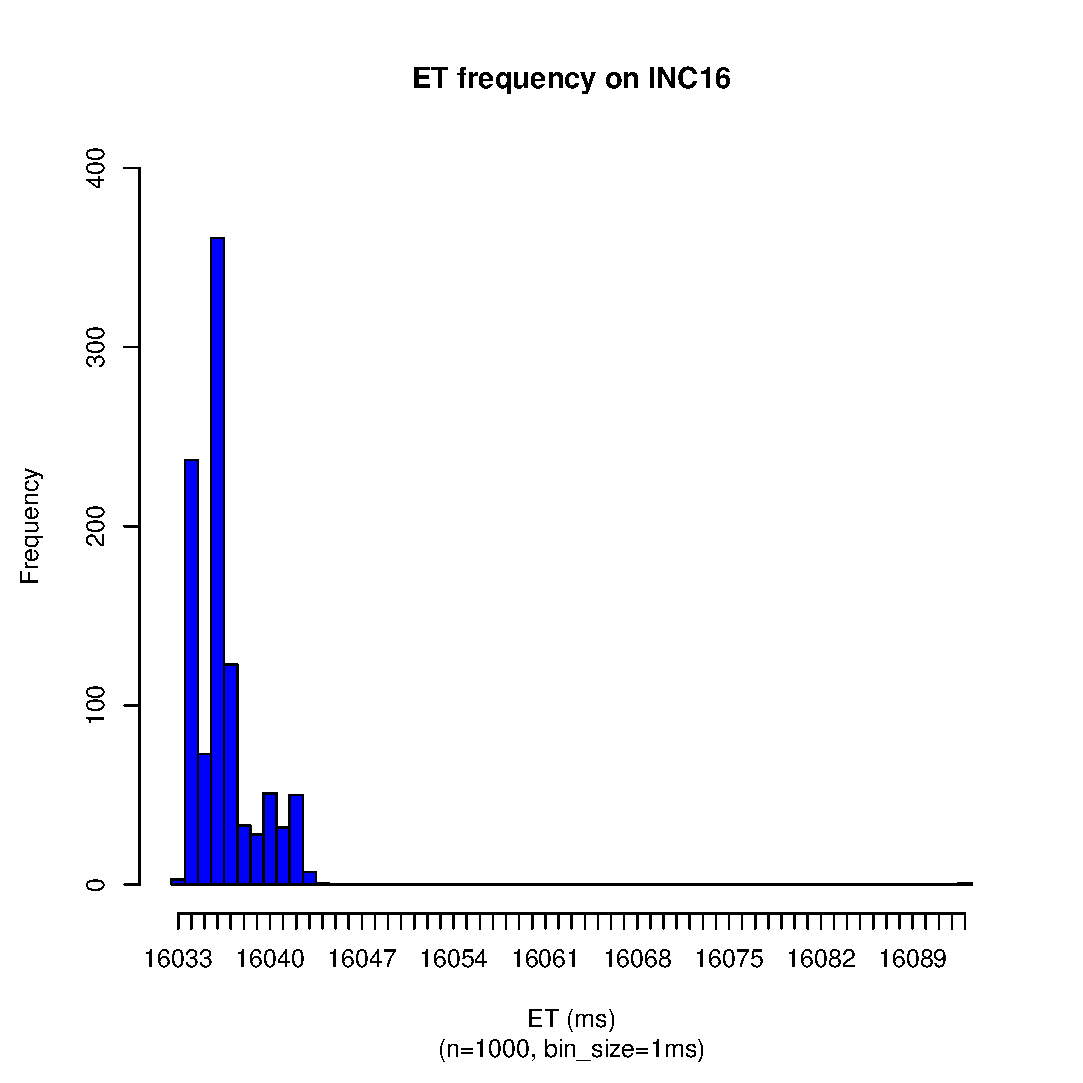
\includegraphics[scale=0.43]{sodb9/16_sec_et_hist_v5.eps}
		\label{fig:inc16_et_hist_v5}
	}
	\subfigure[ET frequency on INC32]{
		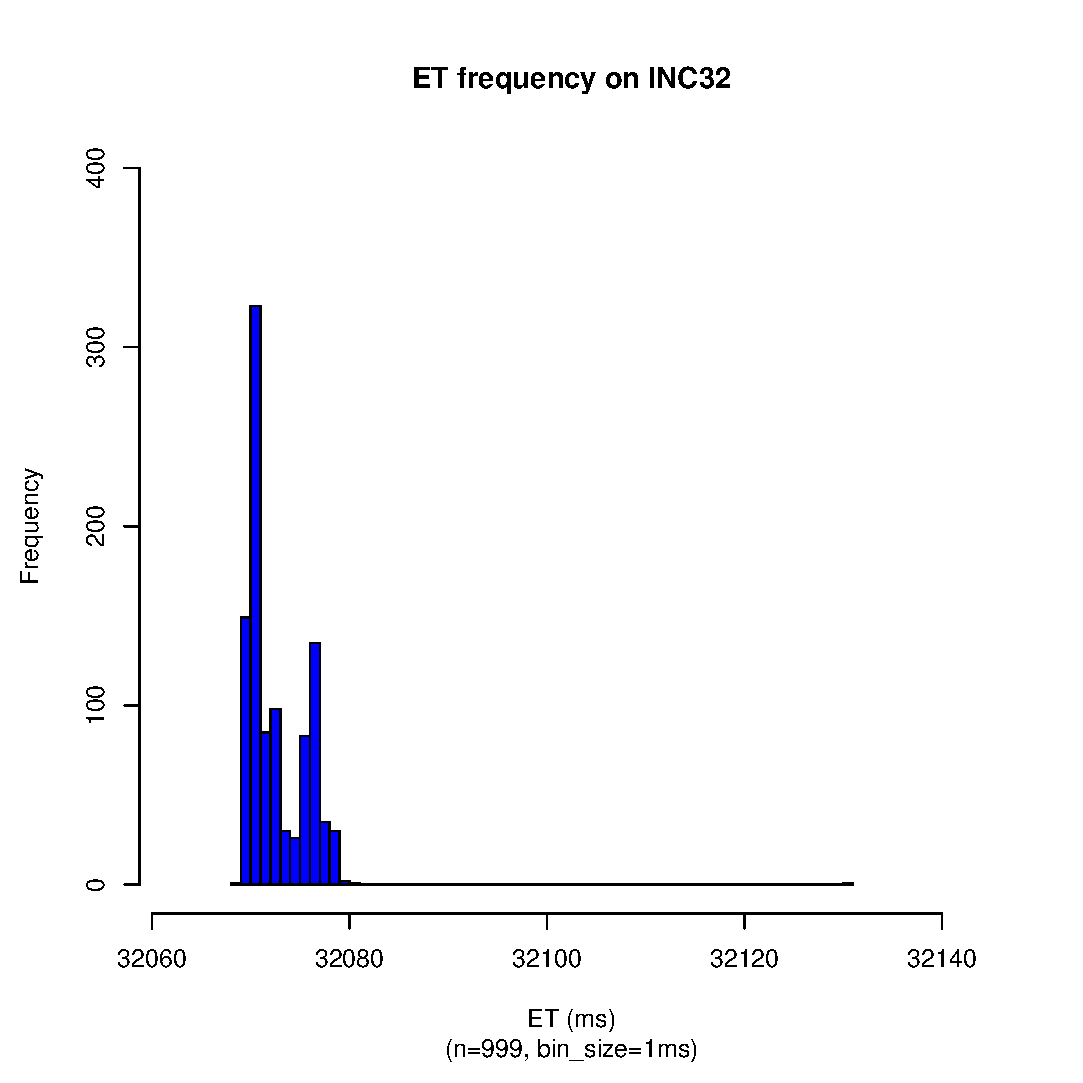
\includegraphics[scale=0.43]{sodb9/32_sec_et_hist_v5.eps}
		\label{fig:inc32_et_hist_v5}
	}
	\subfigure[ET frequency on INC64]{
		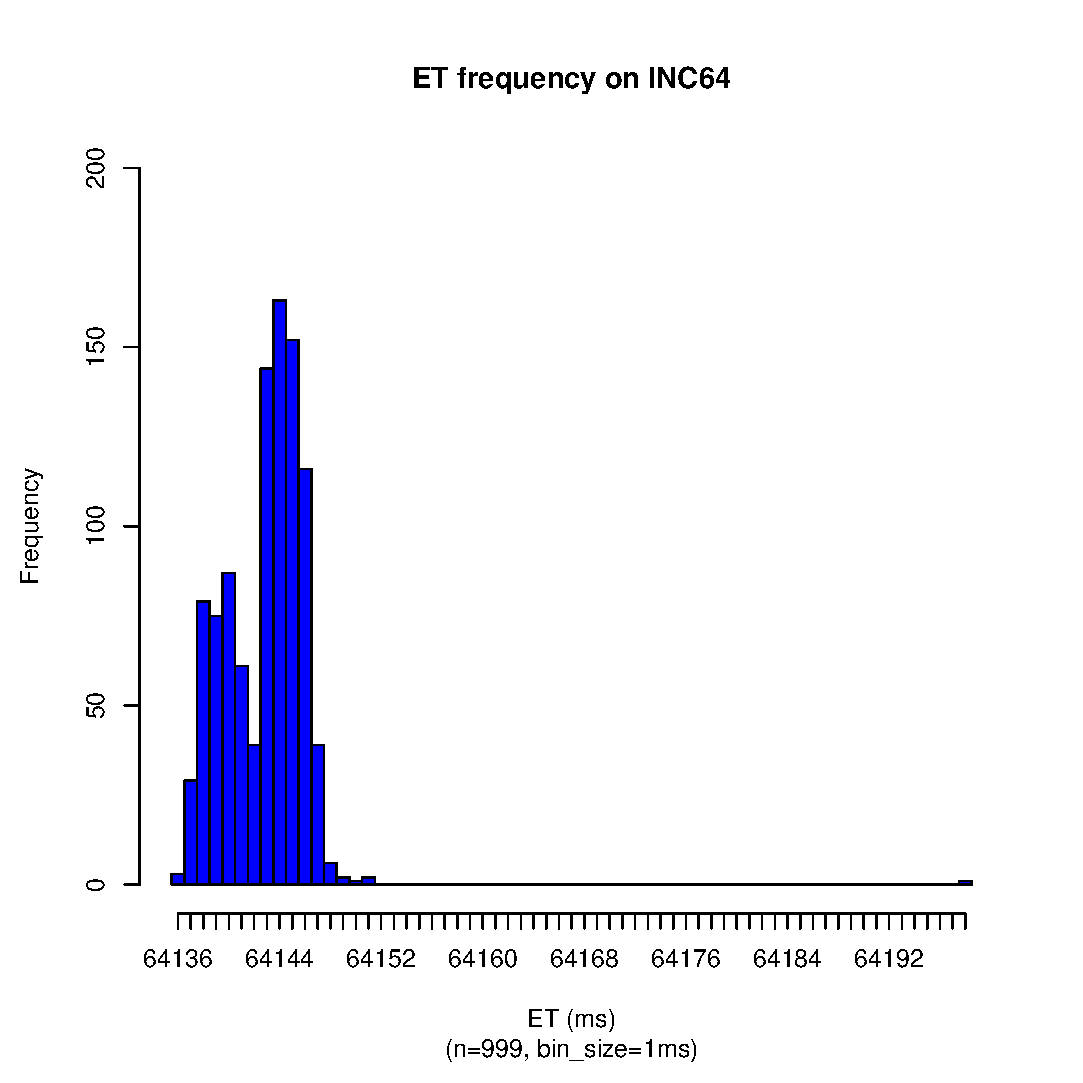
\includegraphics[scale=0.43]{sodb9/64_sec_et_hist_v5.eps}
		\label{fig:inc64_et_hist_v5}
	}
	\caption{ET Histograms of INC16 ... INC64~\label{fig:s9_et_hist2}}
\end{figure}

\begin{figure}[hp!]
	\centering
	\subfigure[ET frequency on INC128]{
		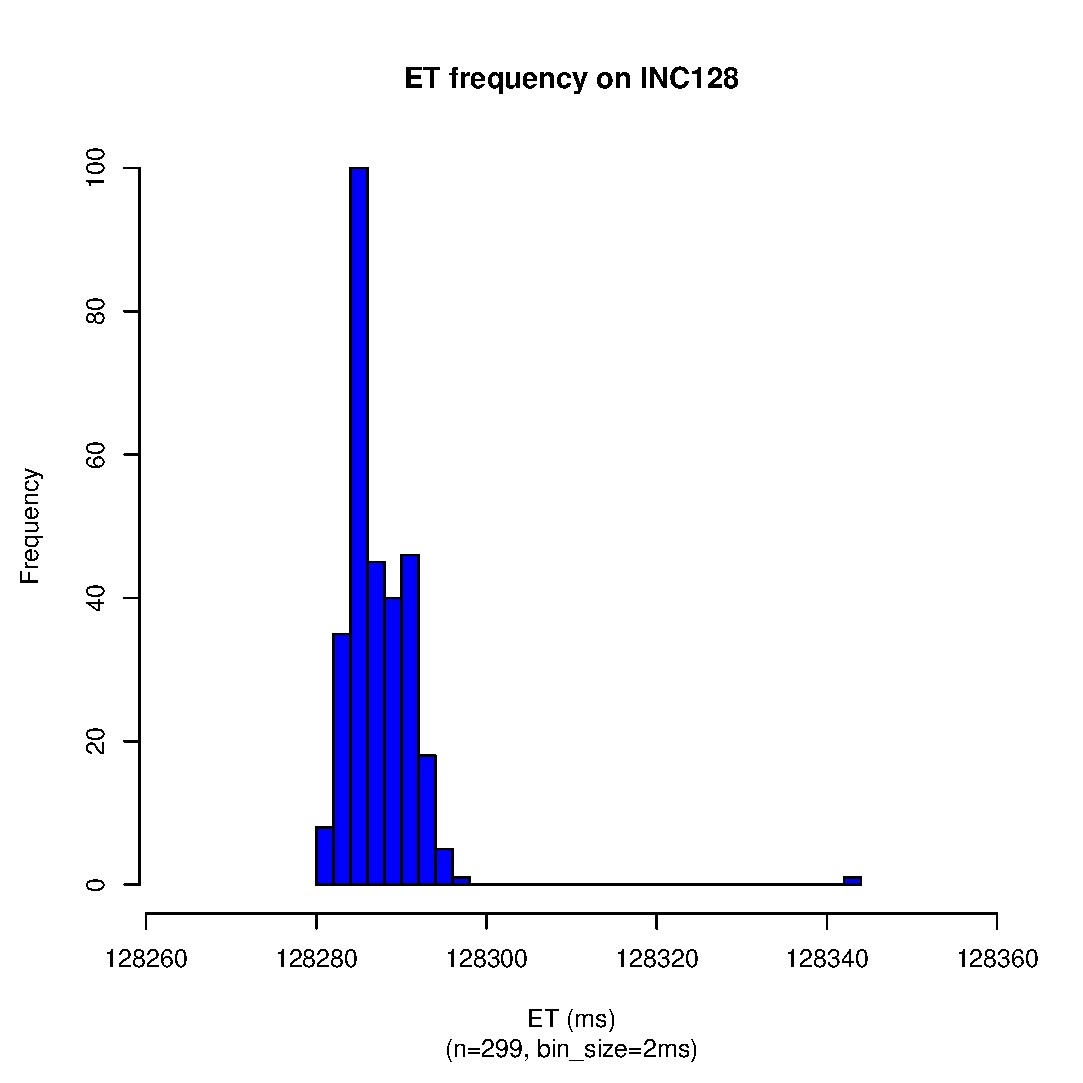
\includegraphics[scale=0.43]{sodb9/128_sec_et_hist_v5.eps}
		\label{fig:inc128_et_hist_v5}
	}
	\subfigure[ET frequency on INC256]{
		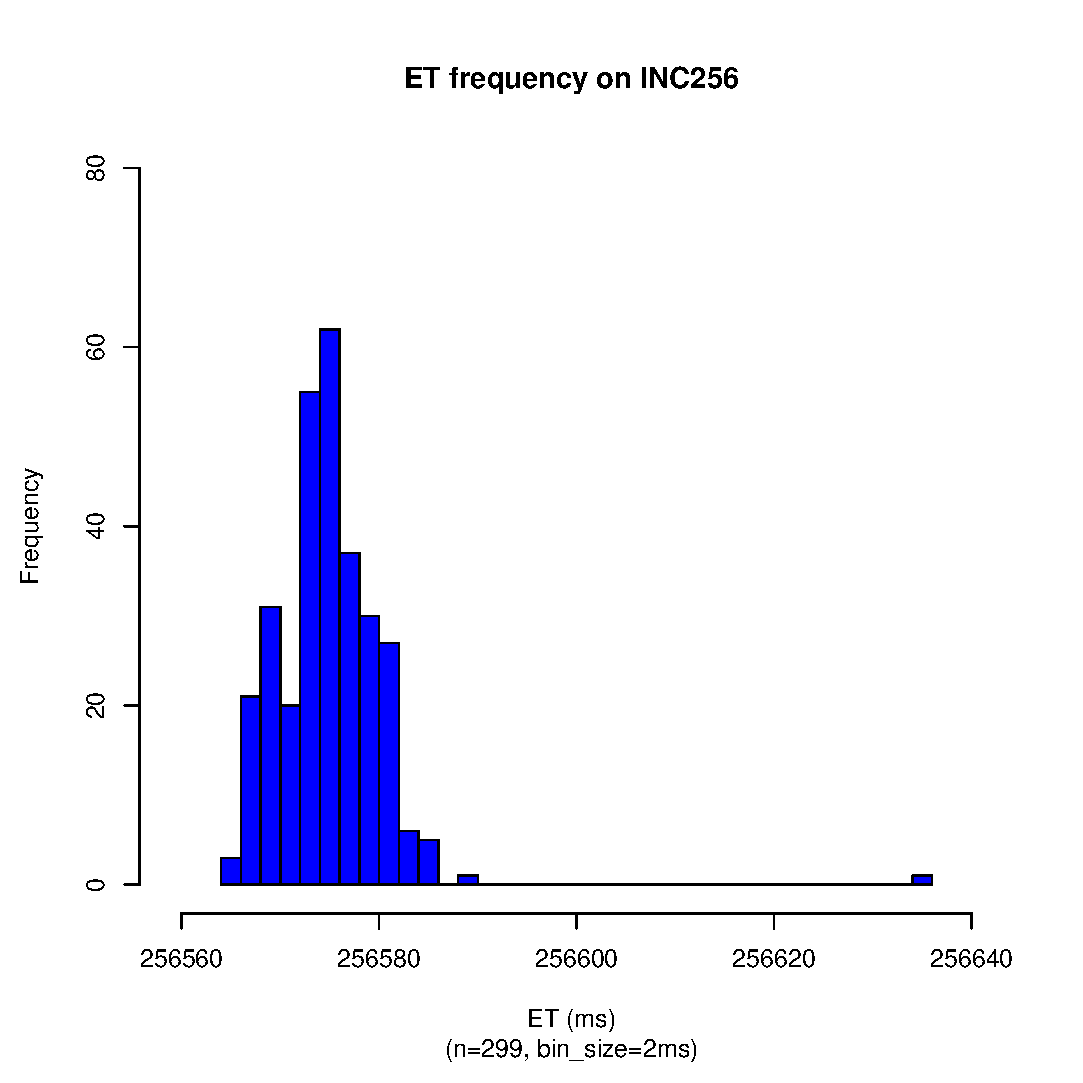
\includegraphics[scale=0.43]{sodb9/256_sec_et_hist_v5.eps}
		\label{fig:inc256_et_hist_v5}
	}
	\subfigure[ET frequency on INC512]{
		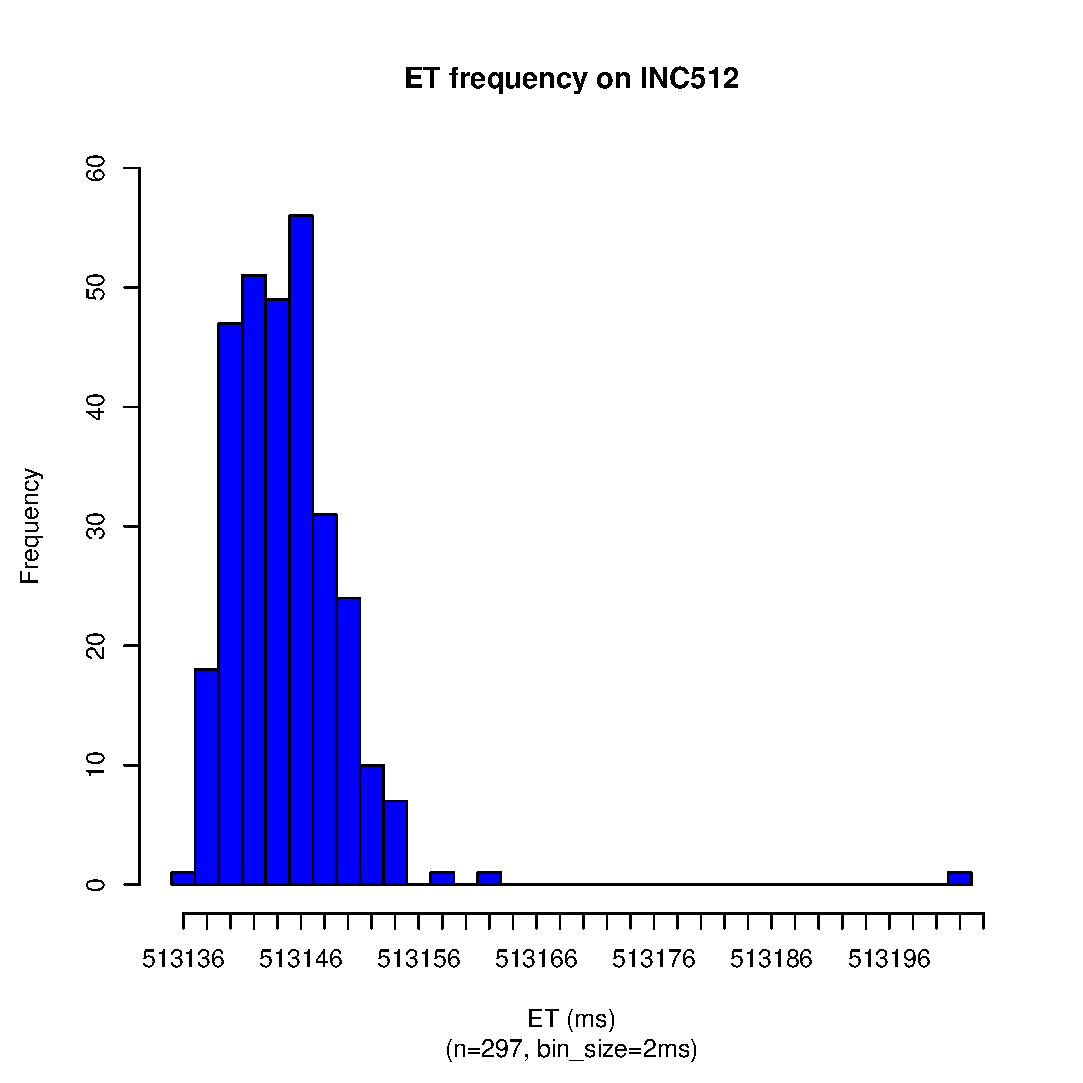
\includegraphics[scale=0.43]{sodb9/512_sec_et_hist_v5.eps}
		\label{fig:inc512_et_hist_v5}
	}
	\subfigure[ET frequency on INC1024]{
		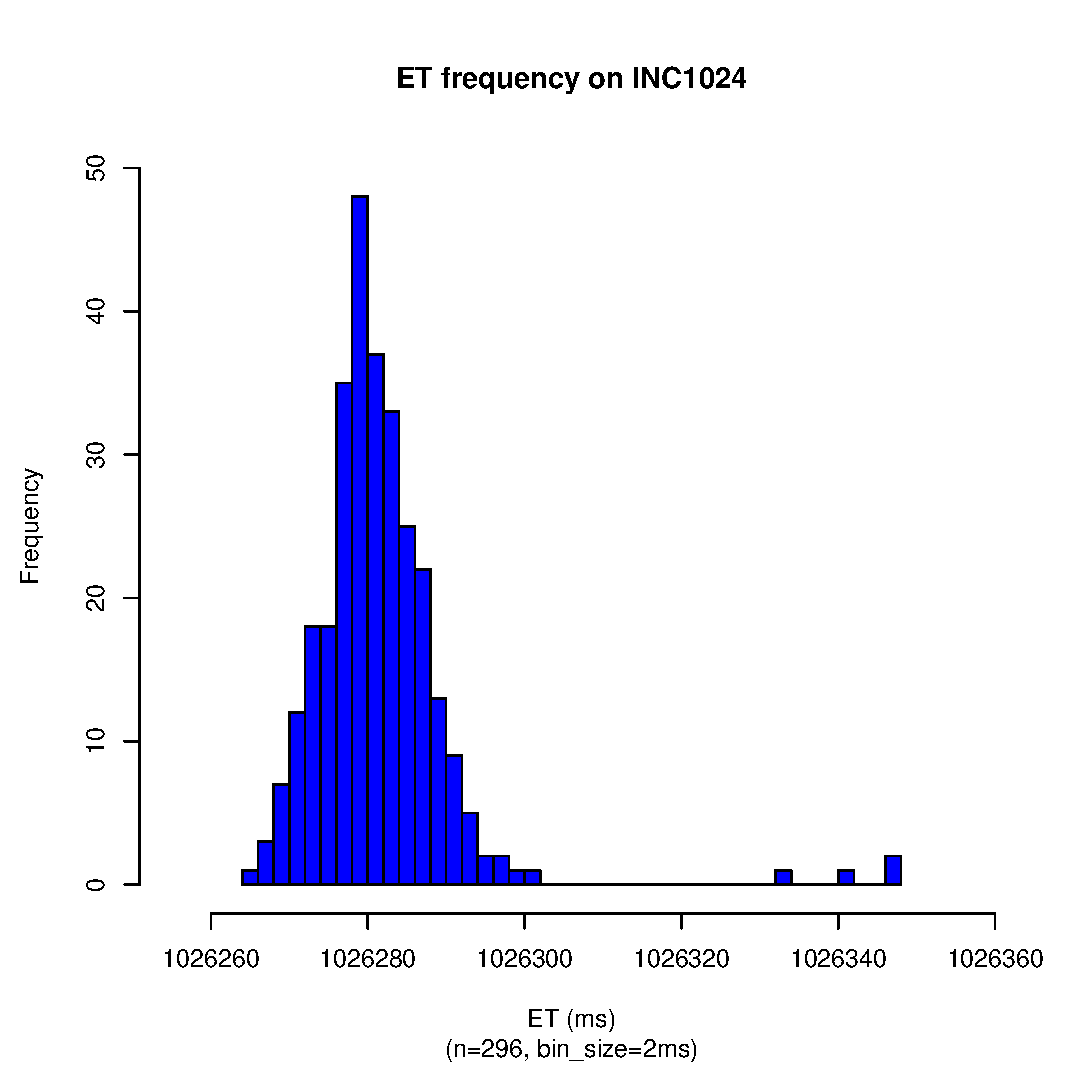
\includegraphics[scale=0.43]{sodb9/1024_sec_et_hist_v5.eps}
		\label{fig:inc1024_et_hist_v5}
	}
	\caption{ET Histograms of INC128 ... INC1024~\label{fig:s9_et_hist3}}
\end{figure}

\pagebreak

\begin{figure}[hp!]
	\centering
	\subfigure[ET frequency on INC2048]{
		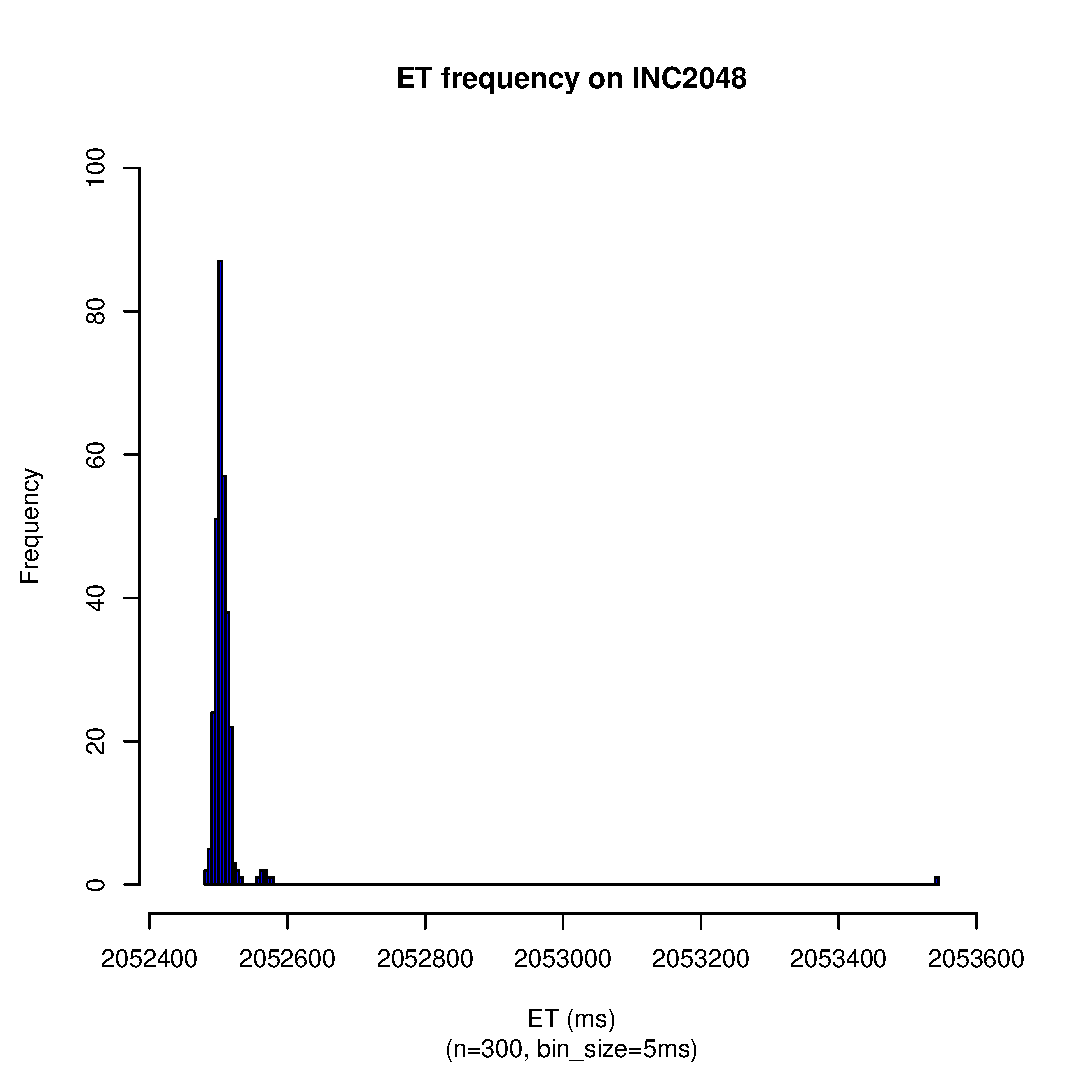
\includegraphics[scale=0.43]{sodb10/2048_sec_et_hist_v5.eps}
		\label{fig:inc2048_et_hist_v5}
	}
	\subfigure[ET frequency on INC4096]{
		\includegraphics[scale=0.43]{sodb12/4096_sec_et_hist_v5.eps}
		\label{fig:inc4096_et_hist_v5}
	}
	\subfigure[ET frequency on INC8192]{
		\includegraphics[scale=0.43]{sodb12/8192_sec_et_hist2_v5.eps}
		\label{fig:inc8192_et_hist_v5}
	}
	\subfigure[ET frequency on INC16384]{
		\includegraphics[scale=0.43]{sodb12/16384_sec_et_hist2_v5.eps}
		\label{fig:inc16384_et_hist_v5}
	}
	\caption{ET Histograms of INC2048 ... INC16384~\label{fig:s9_et_hist4}}
\end{figure}

%\pagebreak
%
%\begin{figure}[hp!]
%	\centering
%	\subfigure[ET frequency on INC8192]{
%		\includegraphics[scale=0.43]{sodb12/8192_sec_et_hist_v5.eps}
%		\label{fig:inc8192_et_hist_all_v5}
%	}
%	\subfigure[ET frequency on INC16384]{
%		\includegraphics[scale=0.43]{sodb12/16384_sec_et_hist_v5.eps}
%		\label{fig:inc16384_et_hist_all_v5}
%	}
%	\caption{ET Histograms of INC8192... INC16384 [combined with 2015's run]~\label{fig:s9_et_hist5}}
%\end{figure}

\newpage

\subsection{PT}

\begin{figure}[hp!]
	\centering
	\subfigure[PT frequency on INC1]{
		\includegraphics[scale=0.43]{sodb9/1_sec_pt_hist_v5.eps}
		\label{fig:inc1_hist_v5}
	}
	\subfigure[PT frequency on INC2]{
		\includegraphics[scale=0.43]{sodb9/2_sec_pt_hist_v5.eps}
		\label{fig:inc2_hist_v5}
	}
	\subfigure[PT frequency on INC4]{
		\includegraphics[scale=0.43]{sodb9/4_sec_pt_hist_v5.eps}
		\label{fig:inc4_hist_v5}
	}
	\subfigure[PT frequency on INC8]{
		\includegraphics[scale=0.43]{sodb9/8_sec_pt_hist_v5.eps}
		\label{fig:inc8_hist_v5}
	}
	\caption{PT Histograms of INC1 ... INC8~\label{fig:s9_pt_hist1}}
\end{figure}

\begin{figure}[hp!]
	\centering
	\subfigure[PT frequency on INC16]{
		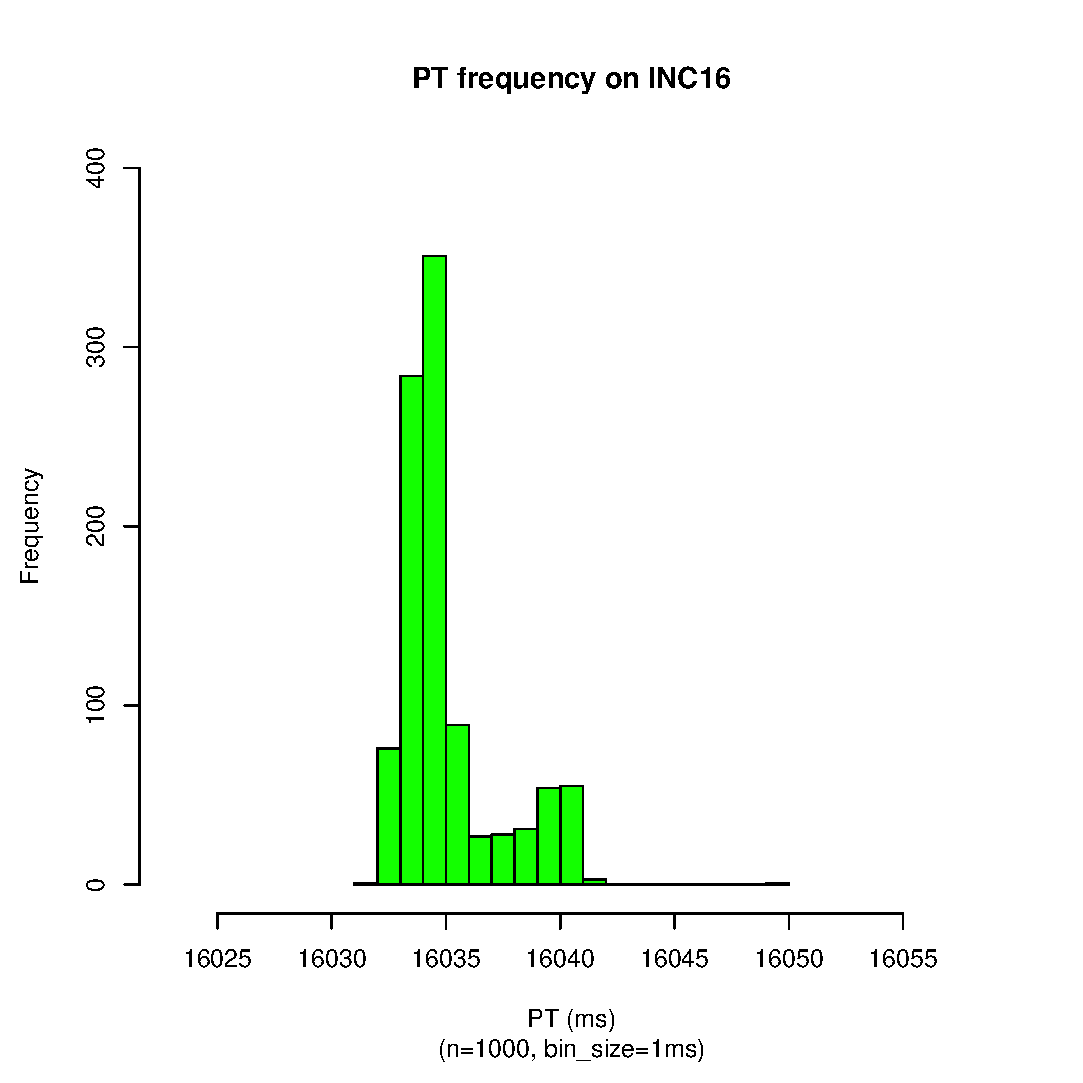
\includegraphics[scale=0.43]{sodb9/16_sec_pt_hist_v5.eps}
		\label{fig:inc16_hist_v5}
	}
	\subfigure[PT frequency on INC32]{
		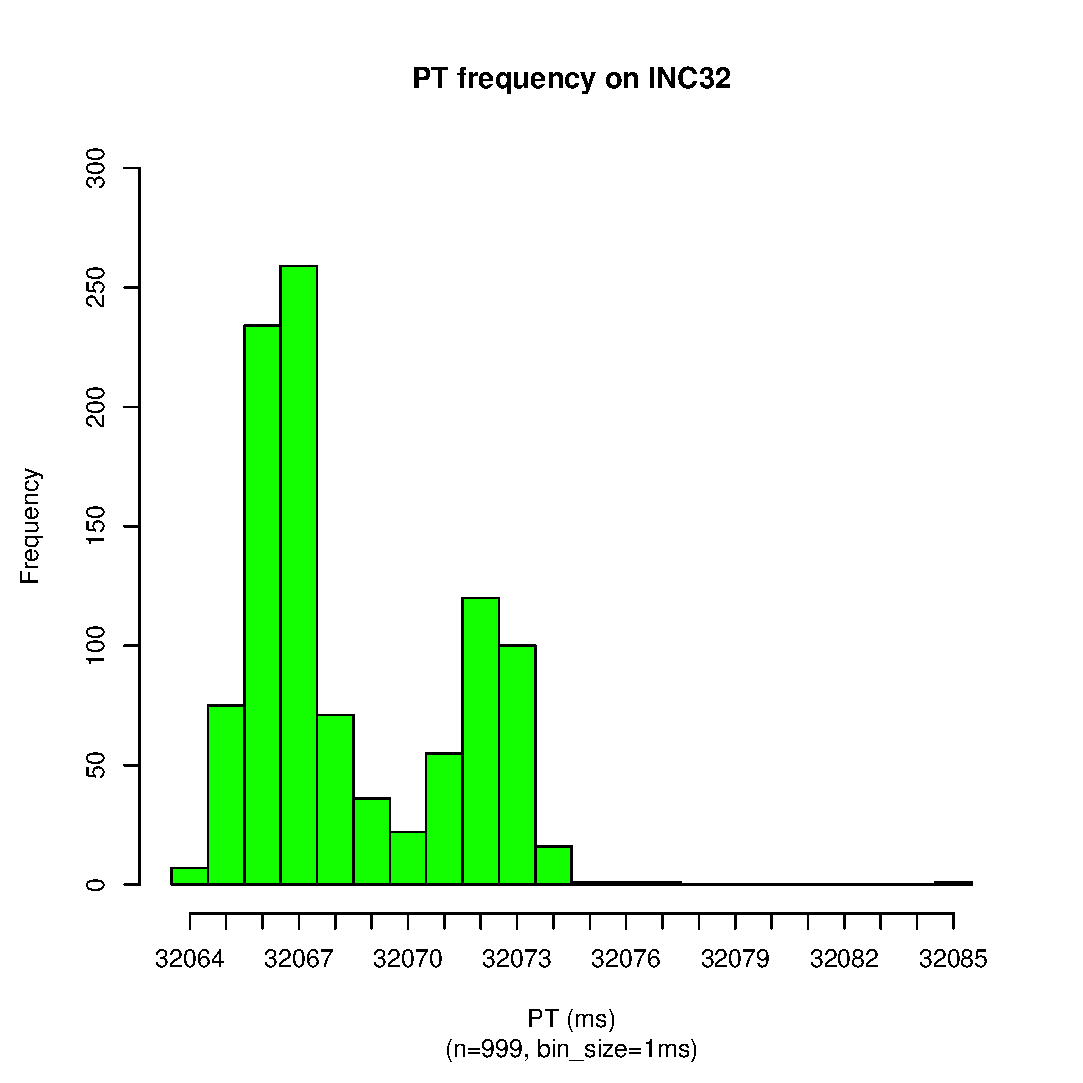
\includegraphics[scale=0.43]{sodb9/32_sec_pt_hist_v5.eps}
		\label{fig:inc32_hist_v5}
	}
	\subfigure[PT frequency on INC64]{
		\includegraphics[scale=0.43]{sodb9/64_sec_pt_hist_v5.eps}
		\label{fig:inc64_hist_v5}
	}
	\caption{PT Histograms of INC16 ... INC64\label{fig:s9_pt_hist2}}
\end{figure}

\begin{figure}[hp!]
	\centering
	\subfigure[PT frequency on INC128]{
		\includegraphics[scale=0.43]{sodb9/128_sec_pt_hist_v5.eps}
		\label{fig:inc128_hist_v5}
	}
	\subfigure[PT frequency on INC256]{
		\includegraphics[scale=0.43]{sodb9/256_sec_pt_hist_v5.eps}
		\label{fig:inc256_hist_v5}
	}
	\subfigure[PT frequency on INC512]{
		\includegraphics[scale=0.43]{sodb9/512_sec_pt_hist_v5.eps}
		\label{fig:inc512_hist_v5}
	}
	\subfigure[PT frequency on INC1024]{
		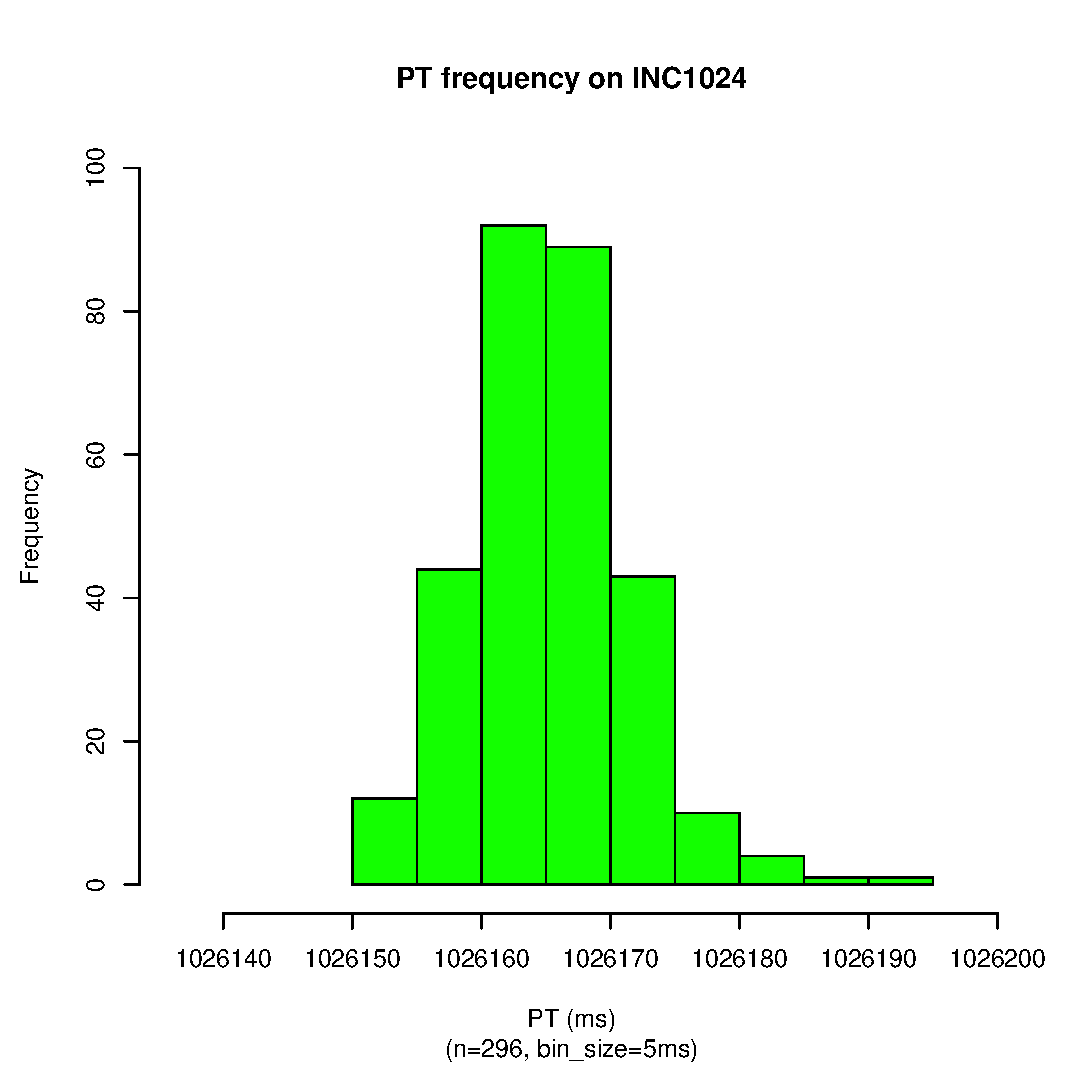
\includegraphics[scale=0.43]{sodb9/1024_sec_pt_hist_v5.eps}
		\label{fig:inc1024_hist_v5}
	}
	\caption{PT Histograms of INC256 ... INC1024~\label{fig:s9_pt_hist3}}
\end{figure}

\begin{figure}[hp!]
	\centering
	\subfigure[PT frequency on INC2048]{
		\includegraphics[scale=0.43]{sodb10/2048_sec_pt_hist_v5.eps}
		\label{fig:inc2048_hist_v5}
	}
	\subfigure[PT frequency on INC4096]{
		\includegraphics[scale=0.43]{sodb12/4096_sec_pt_hist_v5.eps}
		\label{fig:inc4096_hist_v5}
	}
	\subfigure[PT frequency on INC8192]{
		\includegraphics[scale=0.43]{sodb12/8192_sec_pt_hist2_v5.eps}
		\label{fig:inc8192_hist_v5}
	}
	\subfigure[PT frequency on INC16384]{
		\includegraphics[scale=0.43]{sodb12/16384_sec_pt_hist2_v5.eps}
		\label{fig:inc16384_hist_v5}
	}
	\caption{PT Histograms of INC2048 and INC16384~\label{fig:s9_pt_hist4}}
\end{figure}

%\pagebreak
%
%\begin{figure}[hp!]
%	\centering
%	\subfigure[PT frequency on INC8192]{
%		\includegraphics[scale=0.43]{sodb12/8192_sec_pt_hist_v5.eps}
%		\label{fig:inc8192_hist_all_v5}
%	}
%	\subfigure[PT frequency on INC16384]{
%		\includegraphics[scale=0.43]{sodb12/16384_sec_pt_hist_v5.eps}
%		\label{fig:inc16384_hist_all_v5}
%	}
%	\caption{PT Histograms of INC8192 and INC16384 [combined with 2015's run]~\label{fig:s9_pt_hist5}}
%\end{figure}

\pagebreak
\section{Analysis~\label{sec:hist_analysis}} 
In this section we gather all daemons observed and their statistics like minimum PT, maximum PT, average PT, and standard deviation of PT for each bin in Figures~\ref{fig:inc8_et_hist_v5} and~\ref{fig:inc16_et_hist_v5}.

\subsection{INC8}

\begin{table}[h]
\begin{center}
{\scriptsize
\begin{tabular}{l|l|l|l|l|l|l|l} \hline
TASK\_LEN  & BIN (ET) &  DAEMON   & MIN\_PT  &  MAX\_PT  &  AVG\_PT  &   STD\_PT & Counts \\ \hline
INC8     & 8014     & jbd2/md0-8     & 1     & 1     & 1     & 0     & 1\\ \hline
INC8     & 8014     & kslowd000     & 1     & 1     & 1     & 0     & 1\\ \hline
INC8     & 8014     & md0\_raid1     & 1     & 1     & 1     & 0     & 5\\ \hline
INC8     & 8014     & proc\_monitor     & 195     & 200     & 197.05     & 1.43     & 19\\ \hline \hline

INC8     & 8015     & jbd2/md0-8     & 1     & 1     & 1     & 0     & 1\\ \hline
INC8     & 8015     & kslowd001     & 1     & 1     & 1     & 0     & 1\\ \hline
INC8     & 8015     & md0\_raid1     & 1     & 1     & 1     & 0     & 1\\ \hline
INC8     & 8015     & proc\_monitor     & 198     & 198     & 198     & 0     & 4\\ \hline \hline

INC8     & 8016     & jbd2/md0-8     & 1     & 1     & 1     & 0     & 1\\ \hline
INC8     & 8016     & kblockd/0     & 1     & 1     & 1     & 0     & 1\\ \hline
INC8     & 8016     & kslowd000     & 1     & 1     & 1     & 0     & 31\\ \hline
INC8     & 8016     & kslowd001     & 1     & 1     & 1     & 0     & 36\\ \hline
INC8     & 8016     & md0\_raid1     & 1     & 1     & 1     & 0     & 19\\ \hline
INC8     & 8016     & proc\_monitor     & 196     & 198     & 196.72     & .93     & 68\\ \hline \hline

INC8     & 8017     & kslowd000     & 1     & 1     & 1     & 0     & 13\\ \hline
INC8     & 8017     & kslowd001     & 1     & 1     & 1     & 0     & 8\\ \hline
INC8     & 8017     & md0\_raid1     & 1     & 1     & 1     & 0     & 6\\ \hline
INC8     & 8017     & proc\_monitor     & 196     & 198     & 197.55     & .86     & 22\\ \hline \hline

INC8     & 8018     & kslowd000     & 1     & 1     & 1     & 0     & 4\\ \hline
INC8     & 8018     & kslowd001     & 1     & 1     & 1     & 0     & 6\\ \hline
INC8     & 8018     & md0\_raid1     & 1     & 1     & 1     & 0     & 5\\ \hline
INC8     & 8018     & proc\_monitor     & 196     & 198     & 197.4     & .97     & 10\\ \hline \hline

INC8     & 8019     & kslowd000     & 1     & 1     & 1     & 0     & 1\\ \hline
INC8     & 8019     & kslowd001     & 1     & 1     & 1     & 0     & 5\\ \hline
INC8     & 8019     & md0\_raid1     & 1     & 1     & 1     & 0     & 3\\ \hline
INC8     & 8019     & proc\_monitor     & 196     & 198     & 197     & 1.07     & 8\\ \hline \hline

INC8     & 8020     & jbd2/md0-8     & 1     & 1     & 1     & 0     & 1\\ \hline
INC8     & 8020     & kslowd000     & 1     & 1     & 1     & 0     & 3\\ \hline
INC8     & 8020     & kslowd001     & 1     & 1     & 1     & 0     & 1\\ \hline
INC8     & 8020     & md0\_raid1     & 1     & 1     & 1     & 0     & 8\\ \hline
INC8     & 8020     & proc\_monitor     & 196     & 198     & 196.73     & .98     & 33\\ \hline \hline

INC8     & 8021     & kslowd000     & 1     & 1     & 1     & 0     & 6\\ \hline
INC8     & 8021     & kslowd001     & 1     & 1     & 1     & 0     & 4\\ \hline
INC8     & 8021     & md0\_raid1     & 1     & 1     & 1     & 0     & 4\\ \hline
INC8     & 8021     & proc\_monitor     & 196     & 200     & 197.71     & 1.07     & 14\\ \hline \hline

INC8     & 8022     & cifsd     & 1     & 1     & 1     & 0     & 1\\ \hline
INC8     & 8022     & java     & 3     & 14     & 8.5     & 7.78     & 2\\ \hline
INC8     & 8022     & jbd2/md0-8     & 1     & 1     & 1     & 0     & 1\\ \hline
INC8     & 8022     & kslowd000     & 1     & 1     & 1     & 0     & 54\\ \hline
INC8     & 8022     & kslowd001     & 1     & 1     & 1     & 0     & 52\\ \hline
INC8     & 8022     & md0\_raid1     & 1     & 1     & 1     & 0     & 23\\ \hline
INC8     & 8022     & proc\_monitor     & 194     & 198     & 196.94     & 1     & 106\\ \hline \hline

INC8     & 8023     & kslowd000     & 1     & 1     & 1     & 0     & 6\\ \hline
INC8     & 8023     & kslowd001     & 1     & 1     & 1     & 0     & 9\\ \hline
INC8     & 8023     & md0\_raid1     & 1     & 1     & 1     & 0     & 10\\ \hline
INC8     & 8023     & proc\_monitor     & 196     & 198     & 197.87     & .52     & 15\\ \hline \hline

INC8     & 8046     & bash     & 7     & 7     & 7     & 0     & 1\\ \hline
INC8     & 8046     & jbd2/md0-8     & 1     & 1     & 1     & 0     & 1\\ \hline
INC8     & 8046     & kslowd000     & 1     & 1     & 1     & 0     & 1\\ \hline
INC8     & 8046     & proc\_monitor     & 198     & 198     & 198     & 0     & 1\\ \hline
INC8     & 8046     & sshd     & 1     & 14     & 5.33     & 7.51     & 3\\ \hline \hline
\end{tabular}
}
\end{center}
\caption{Daemons observed from the INC8 run~\label{tab:inc8_daemons}}
\end{table}

\pagebreak

\subsection{INC16}

\begin{table}[h]
\begin{center}
{\scriptsize
\begin{tabular}{l|l|l|l|l|l|l|l} \hline
TASK\_LEN  & BIN (ET) &  DAEMON   & MIN\_PT  &  MAX\_PT  &  AVG\_PT  &   STD\_PT & Counts \\ \hline
INC16     & 16034     & jbd2/md0-8     & 1     & 1     & 1     & 0     & 1\\ \hline
INC16     & 16034     & kslowd000     & 1     & 1     & 1     & 0     & 30\\ \hline
INC16     & 16034     & kslowd001     & 1     & 1     & 1     & 0     & 28\\ \hline
INC16     & 16034     & md0\_raid1     & 1     & 1     & 1     & 0     & 13\\ \hline
INC16     & 16034     & proc\_monitor     & 196     & 198     & 196.58     & .89     & 57\\ \hline \hline

INC16     & 16035     & java     & 2     & 3     & 2.75     & .5     & 4\\ \hline
INC16     & 16035     & kslowd000     & 1     & 1     & 1     & 0     & 15\\ \hline
INC16     & 16035     & kslowd001     & 1     & 1     & 1     & 0     & 19\\ \hline
INC16     & 16035     & md0\_raid1     & 1     & 1     & 1     & 0     & 7\\ \hline
INC16     & 16035     & proc\_monitor     & 196     & 200     & 197.47     & 1.13     & 34\\ \hline \hline

INC16     & 16036     & java     & 2     & 3     & 2.5     & .71     & 2\\ \hline
INC16     & 16036     & jbd2/md0-8     & 1     & 1     & 1     & 0     & 3\\ \hline
INC16     & 16036     & kslowd000     & 1     & 2     & 1.01     & .11     & 90\\ \hline
INC16     & 16036     & kslowd001     & 1     & 2     & 1.01     & .11     & 90\\ \hline
INC16     & 16036     & md0\_raid1     & 1     & 1     & 1     & 0     & 23\\ \hline
INC16     & 16036     & proc\_monitor     & 196     & 200     & 196.81     & 1.1     & 94\\ \hline \hline

INC16     & 16037     & cifsd     & 1     & 1     & 1     & 0     & 1\\ \hline
INC16     & 16037     & jbd2/md0-8     & 1     & 1     & 1     & 0     & 1\\ \hline
INC16     & 16037     & kslowd000     & 1     & 2     & 1.02     & .13     & 55\\ \hline
INC16     & 16037     & kslowd001     & 1     & 1     & 1     & 0     & 54\\ \hline
INC16     & 16037     & md0\_raid1     & 1     & 1     & 1     & 0     & 16\\ \hline
INC16     & 16037     & proc\_monitor     & 196     & 198     & 197.53     & .86     & 55\\ \hline \hline

INC16     & 16038     & cifsd     & 1     & 1     & 1     & 0     & 1\\ \hline
INC16     & 16038     & khugepaged     & 1     & 2     & 1.5     & .71     & 2\\ \hline
INC16     & 16038     & kslowd000     & 1     & 1     & 1     & 0     & 9\\ \hline
INC16     & 16038     & kslowd001     & 1     & 1     & 1     & 0     & 8\\ \hline
INC16     & 16038     & proc\_monitor     & 196     & 198     & 197.56     & .88     & 9\\ \hline \hline

INC16     & 16039     & kslowd000     & 1     & 1     & 1     & 0     & 9\\ \hline
INC16     & 16039     & kslowd001     & 1     & 1     & 1     & 0     & 10\\ \hline
INC16     & 16039     & md0\_raid1     & 1     & 1     & 1     & 0     & 7\\ \hline
INC16     & 16039     & proc\_monitor     & 196     & 200     & 197.31     & 1.38     & 13\\ \hline \hline

INC16     & 16040     & khugepaged     & 1     & 1     & 1     & 0     & 1\\ \hline
INC16     & 16040     & kslowd000     & 1     & 1     & 1     & 0     & 8\\ \hline
INC16     & 16040     & kslowd001     & 1     & 1     & 1     & 0     & 8\\ \hline
INC16     & 16040     & md0\_raid1     & 1     & 1     & 1     & 0     & 1\\ \hline
INC16     & 16040     & proc\_monitor     & 195     & 198     & 196.64     & 1.12     & 11\\ \hline \hline

INC16     & 16041     & kslowd000     & 1     & 1     & 1     & 0     & 5\\ \hline
INC16     & 16041     & kslowd001     & 1     & 1     & 1     & 0     & 3\\ \hline
INC16     & 16041     & md0\_raid1     & 1     & 1     & 1     & 0     & 1\\ \hline
INC16     & 16041     & proc\_monitor     & 198     & 198     & 198     & 0     & 6\\ \hline \hline

INC16     & 16042     & java     & 3     & 16     & 9.5     & 9.19     & 2\\ \hline
INC16     & 16042     & kblockd/0     & 1     & 1     & 1     & 0     & 1\\ \hline
INC16     & 16042     & kslowd000     & 1     & 1     & 1     & 0     & 17\\ \hline
INC16     & 16042     & kslowd001     & 1     & 1     & 1     & 0     & 17\\ \hline
INC16     & 16042     & md0\_raid1     & 1     & 1     & 1     & 0     & 5\\ \hline
INC16     & 16042     & proc\_monitor     & 196     & 200     & 197.06     & 1.39     & 17\\ \hline \hline

INC16     & 16043     & jbd2/md0-8     & 1     & 1     & 1     & 0     & 1\\ \hline
INC16     & 16043     & kslowd000     & 1     & 1     & 1     & 0     & 4\\ \hline
INC16     & 16043     & kslowd001     & 1     & 1     & 1     & 0     & 4\\ \hline
INC16     & 16043     & md0\_raid1     & 1     & 1     & 1     & 0     & 1\\ \hline
INC16     & 16043     & proc\_monitor     & 196     & 198     & 197.5     & 1     & 4\\ \hline \hline

\end{tabular}
}
\end{center}
\caption{Daemons observed from the INC16 run~\label{tab:inc16_daemons}}
\end{table}

\section{Histograms~\label{sec:sodb9_hist}} 
This section exhibits histograms on the EMPv5 data obtained when 
the task length of INC increases from 1 second to 2048 seconds. 
The detailed description of the base data is from Table~\ref{tab:exp_notes}.

\subsection{ET}

\begin{figure}[hp!]
	\centering
	\subfigure[ET frequency on INC1]{
		\includegraphics[scale=0.43]{sodb9/1_sec_et_hist_v5.eps}
		\label{fig:inc1_et_hist_v5}
	}
	\subfigure[ET frequency on INC2]{
		\includegraphics[scale=0.43]{sodb9/2_sec_et_hist_v5.eps}
		\label{fig:inc2_et_hist_v5}
	}
	\subfigure[ET frequency on INC4]{
		\includegraphics[scale=0.43]{sodb9/4_sec_et_hist_v5.eps}
		\label{fig:inc4_et_hist_v5}
	}
	\subfigure[ET frequency on INC8]{
		\includegraphics[scale=0.43]{sodb9/8_sec_et_hist_v5.eps}
		\label{fig:inc8_et_hist_v5}
	}
	\caption{ET Histograms of INC1 ... INC8~\label{fig:s9_et_hist1}}
\end{figure}

\begin{figure}[hp!]
	\centering
	\subfigure[ET frequency on INC16]{
		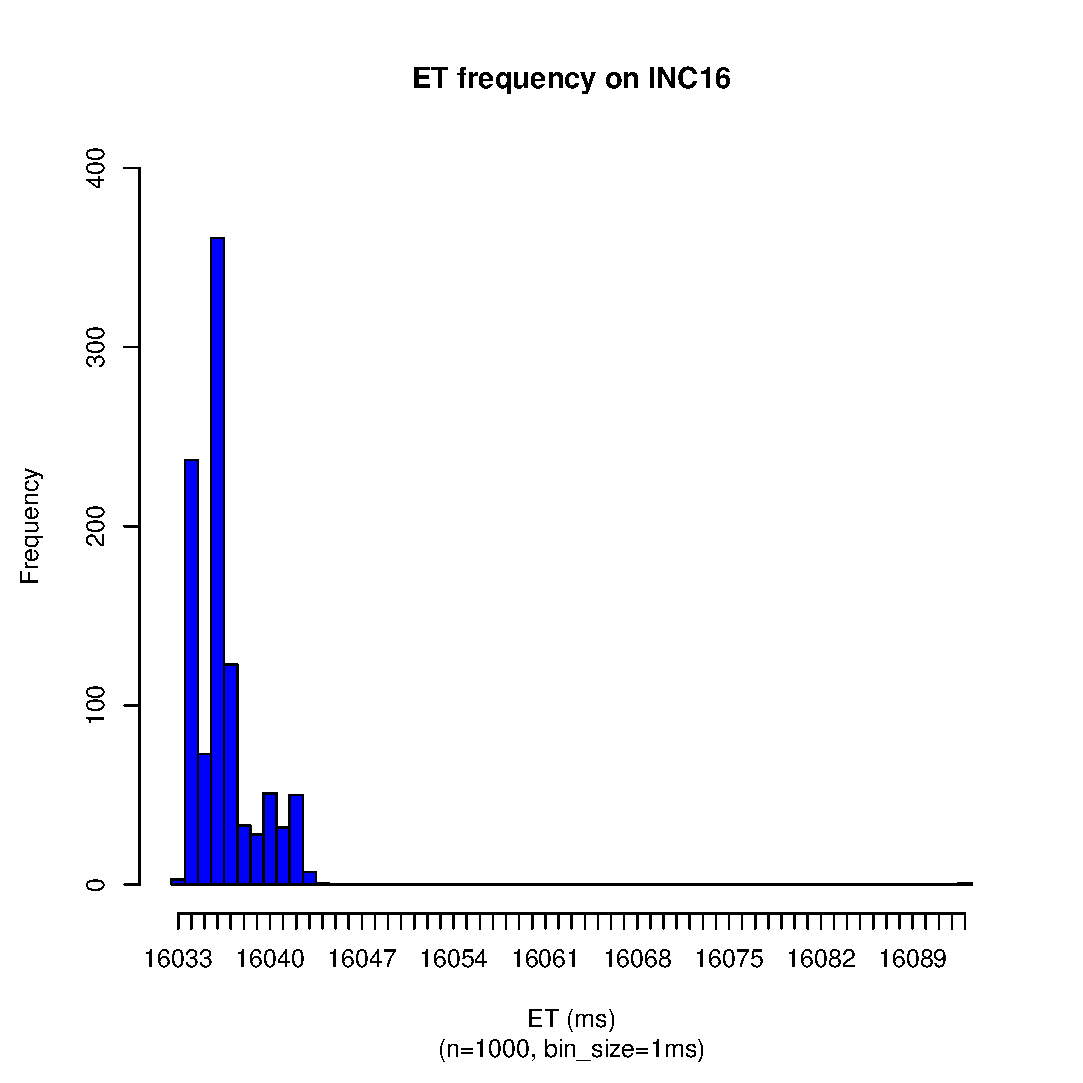
\includegraphics[scale=0.43]{sodb9/16_sec_et_hist_v5.eps}
		\label{fig:inc16_et_hist_v5}
	}
	\subfigure[ET frequency on INC32]{
		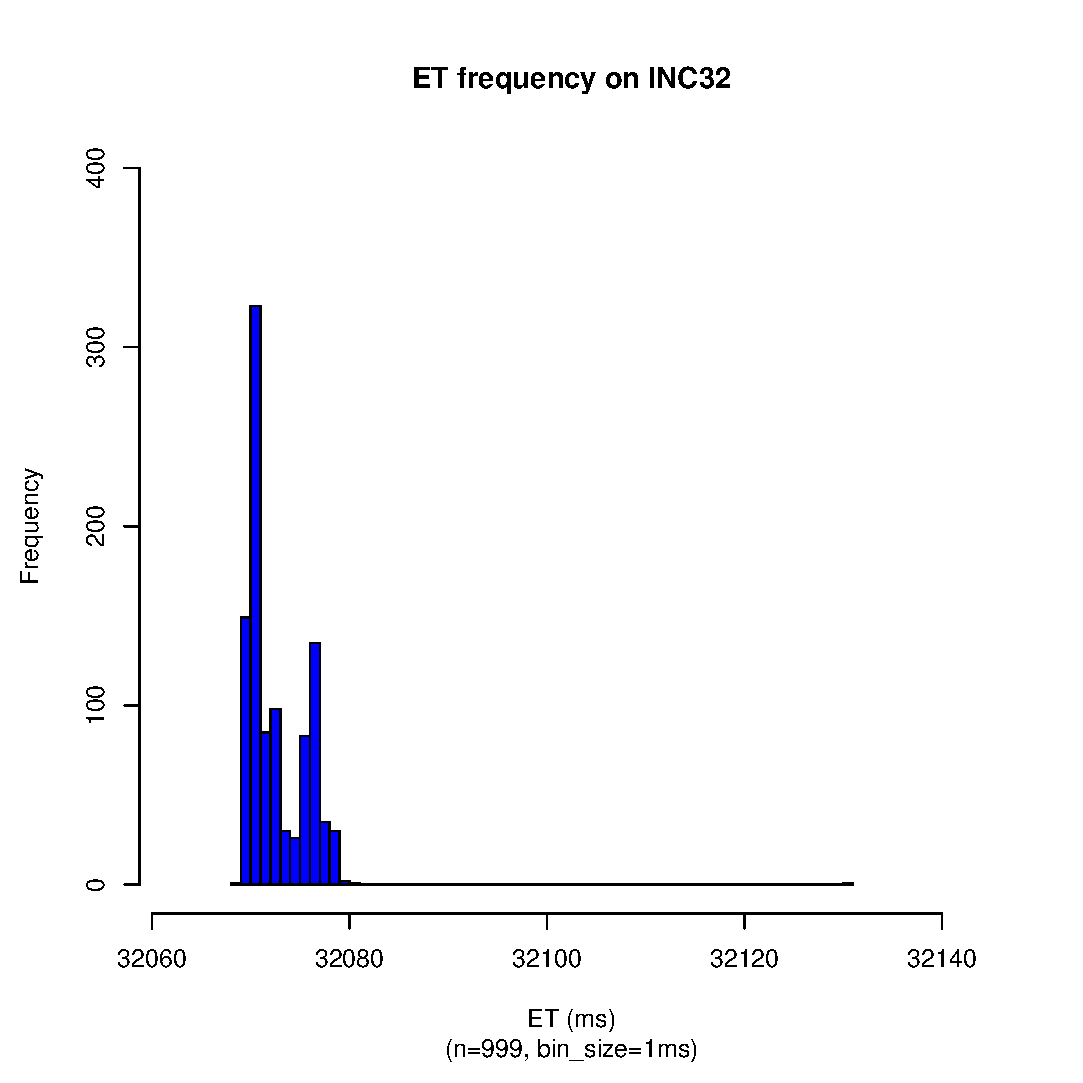
\includegraphics[scale=0.43]{sodb9/32_sec_et_hist_v5.eps}
		\label{fig:inc32_et_hist_v5}
	}
	\subfigure[ET frequency on INC64]{
		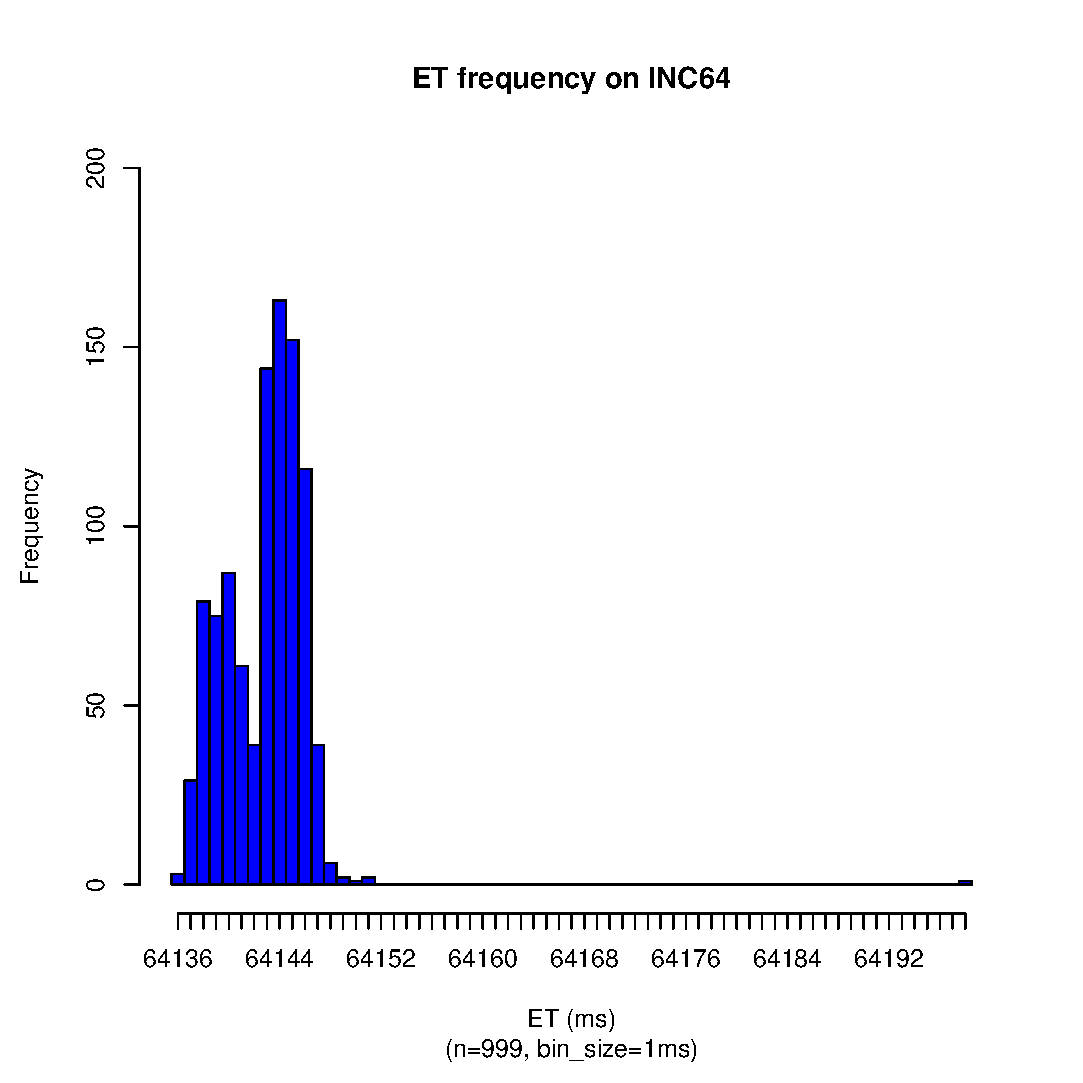
\includegraphics[scale=0.43]{sodb9/64_sec_et_hist_v5.eps}
		\label{fig:inc64_et_hist_v5}
	}
	\caption{ET Histograms of INC16 ... INC64~\label{fig:s9_et_hist2}}
\end{figure}

\begin{figure}[hp!]
	\centering
	\subfigure[ET frequency on INC128]{
		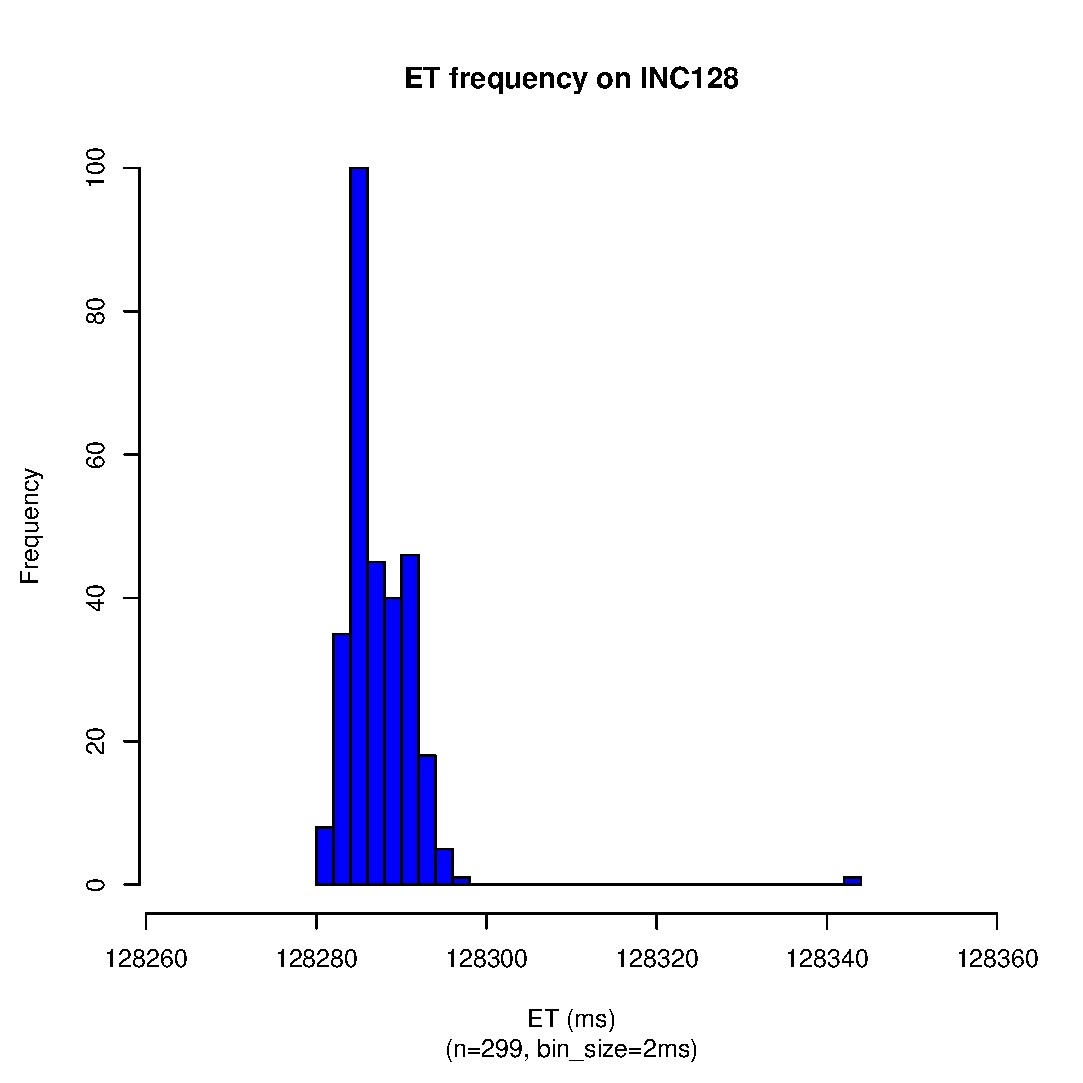
\includegraphics[scale=0.43]{sodb9/128_sec_et_hist_v5.eps}
		\label{fig:inc128_et_hist_v5}
	}
	\subfigure[ET frequency on INC256]{
		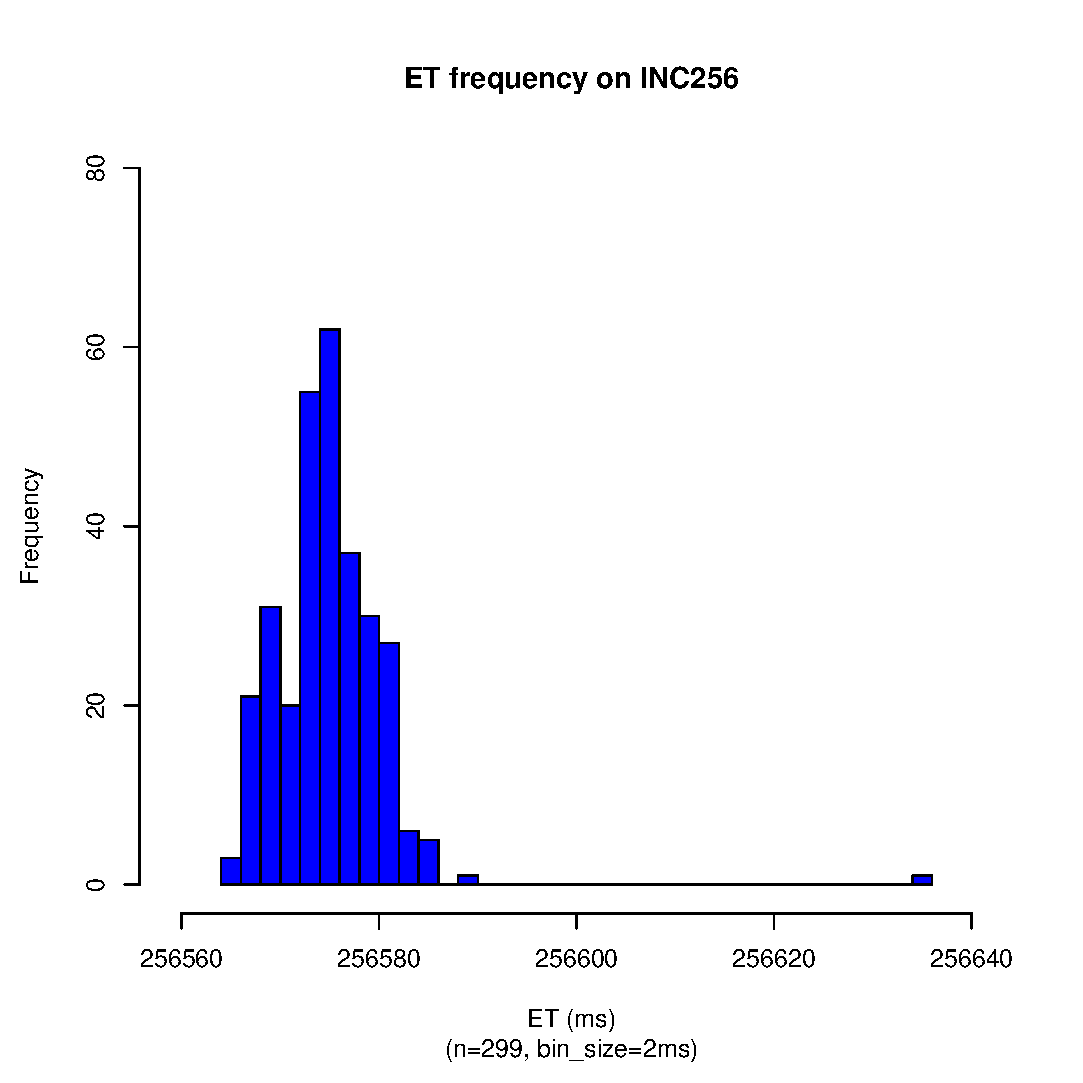
\includegraphics[scale=0.43]{sodb9/256_sec_et_hist_v5.eps}
		\label{fig:inc256_et_hist_v5}
	}
	\subfigure[ET frequency on INC512]{
		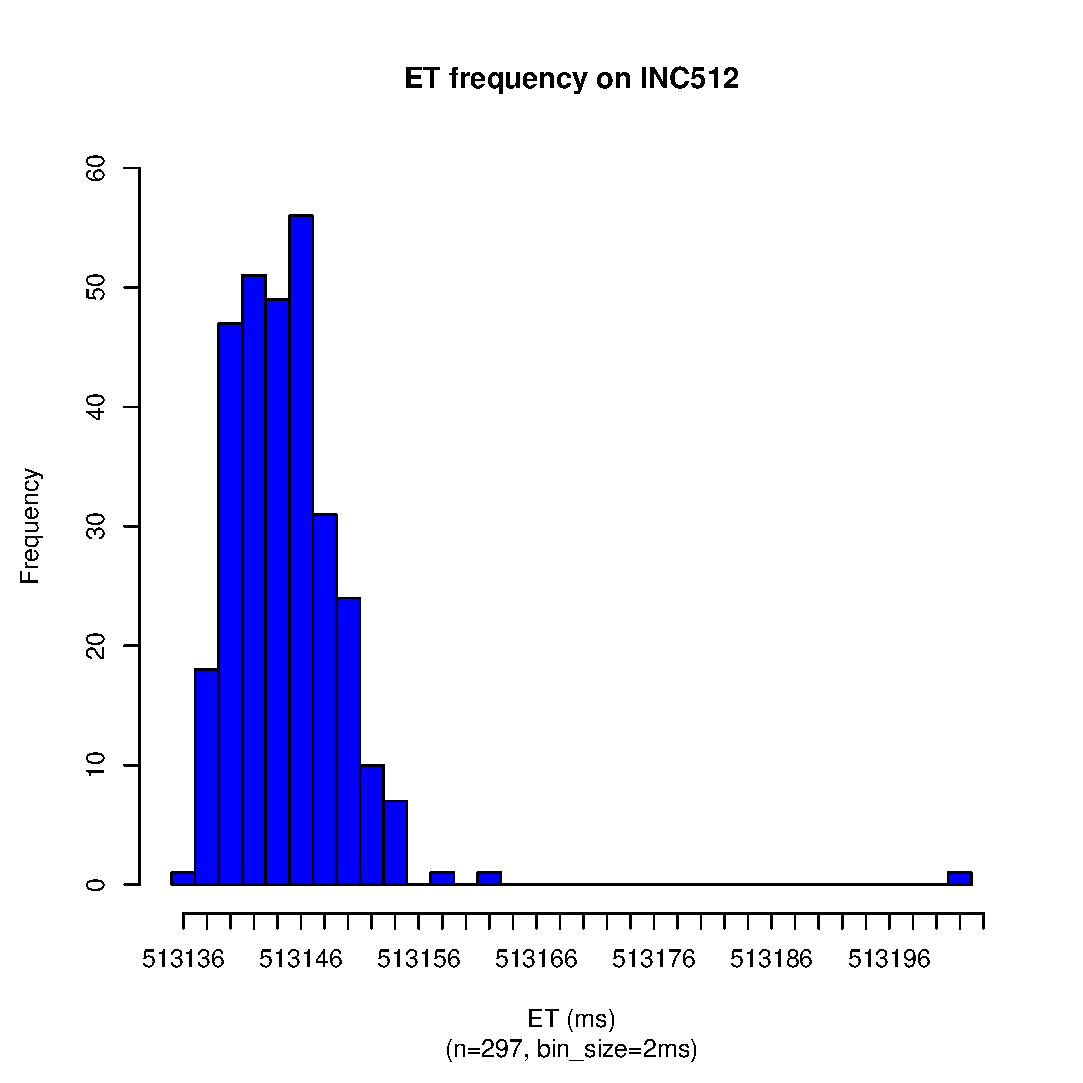
\includegraphics[scale=0.43]{sodb9/512_sec_et_hist_v5.eps}
		\label{fig:inc512_et_hist_v5}
	}
	\subfigure[ET frequency on INC1024]{
		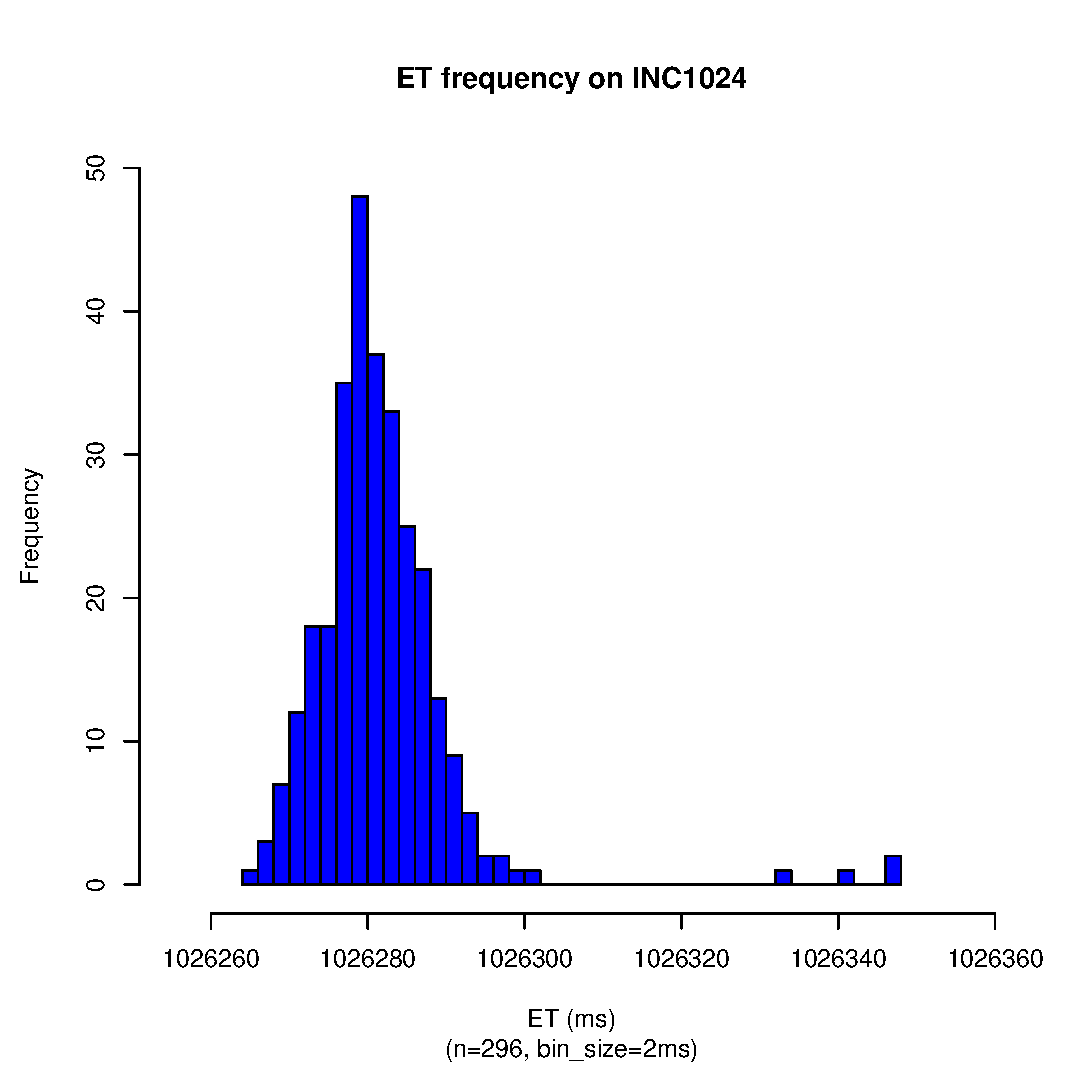
\includegraphics[scale=0.43]{sodb9/1024_sec_et_hist_v5.eps}
		\label{fig:inc1024_et_hist_v5}
	}
	\caption{ET Histograms of INC128 ... INC1024~\label{fig:s9_et_hist3}}
\end{figure}

\pagebreak

\begin{figure}[hp!]
	\centering
	\subfigure[ET frequency on INC2048]{
		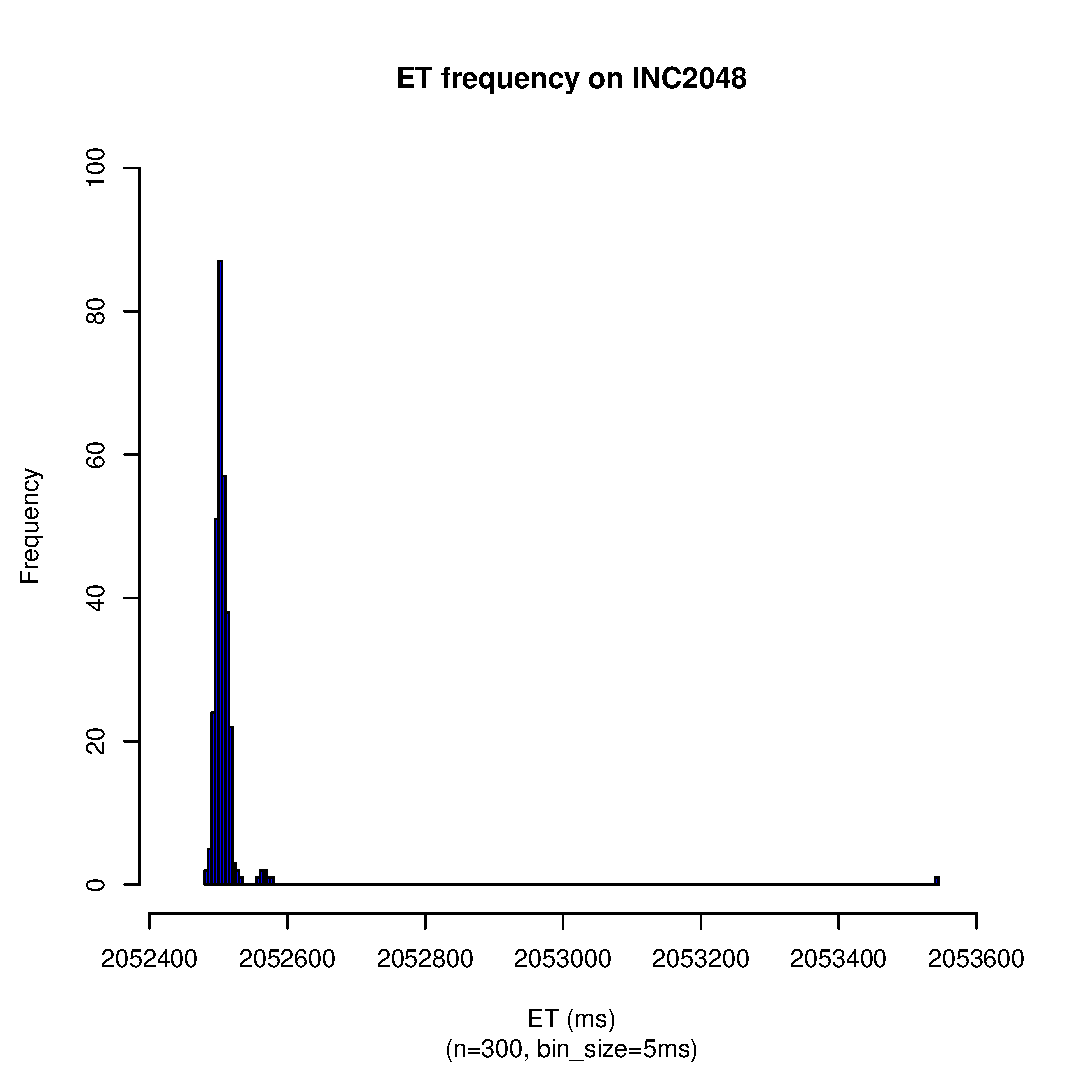
\includegraphics[scale=0.43]{sodb10/2048_sec_et_hist_v5.eps}
		\label{fig:inc2048_et_hist_v5}
	}
	\subfigure[ET frequency on INC4096]{
		\includegraphics[scale=0.43]{sodb12/4096_sec_et_hist_v5.eps}
		\label{fig:inc4096_et_hist_v5}
	}
	\subfigure[ET frequency on INC8192]{
		\includegraphics[scale=0.43]{sodb12/8192_sec_et_hist2_v5.eps}
		\label{fig:inc8192_et_hist_v5}
	}
	\subfigure[ET frequency on INC16384]{
		\includegraphics[scale=0.43]{sodb12/16384_sec_et_hist2_v5.eps}
		\label{fig:inc16384_et_hist_v5}
	}
	\caption{ET Histograms of INC2048 ... INC16384~\label{fig:s9_et_hist4}}
\end{figure}

%\pagebreak
%
%\begin{figure}[hp!]
%	\centering
%	\subfigure[ET frequency on INC8192]{
%		\includegraphics[scale=0.43]{sodb12/8192_sec_et_hist_v5.eps}
%		\label{fig:inc8192_et_hist_all_v5}
%	}
%	\subfigure[ET frequency on INC16384]{
%		\includegraphics[scale=0.43]{sodb12/16384_sec_et_hist_v5.eps}
%		\label{fig:inc16384_et_hist_all_v5}
%	}
%	\caption{ET Histograms of INC8192... INC16384 [combined with 2015's run]~\label{fig:s9_et_hist5}}
%\end{figure}

\newpage

\subsection{PT}

\begin{figure}[hp!]
	\centering
	\subfigure[PT frequency on INC1]{
		\includegraphics[scale=0.43]{sodb9/1_sec_pt_hist_v5.eps}
		\label{fig:inc1_hist_v5}
	}
	\subfigure[PT frequency on INC2]{
		\includegraphics[scale=0.43]{sodb9/2_sec_pt_hist_v5.eps}
		\label{fig:inc2_hist_v5}
	}
	\subfigure[PT frequency on INC4]{
		\includegraphics[scale=0.43]{sodb9/4_sec_pt_hist_v5.eps}
		\label{fig:inc4_hist_v5}
	}
	\subfigure[PT frequency on INC8]{
		\includegraphics[scale=0.43]{sodb9/8_sec_pt_hist_v5.eps}
		\label{fig:inc8_hist_v5}
	}
	\caption{PT Histograms of INC1 ... INC8~\label{fig:s9_pt_hist1}}
\end{figure}

\begin{figure}[hp!]
	\centering
	\subfigure[PT frequency on INC16]{
		\includegraphics[scale=0.43]{sodb9/16_sec_pt_hist_v5.eps}
		\label{fig:inc16_hist_v5}
	}
	\subfigure[PT frequency on INC32]{
		\includegraphics[scale=0.43]{sodb9/32_sec_pt_hist_v5.eps}
		\label{fig:inc32_hist_v5}
	}
	\subfigure[PT frequency on INC64]{
		\includegraphics[scale=0.43]{sodb9/64_sec_pt_hist_v5.eps}
		\label{fig:inc64_hist_v5}
	}
	\caption{PT Histograms of INC16 ... INC64\label{fig:s9_pt_hist2}}
\end{figure}

\begin{figure}[hp!]
	\centering
	\subfigure[PT frequency on INC128]{
		\includegraphics[scale=0.43]{sodb9/128_sec_pt_hist_v5.eps}
		\label{fig:inc128_hist_v5}
	}
	\subfigure[PT frequency on INC256]{
		\includegraphics[scale=0.43]{sodb9/256_sec_pt_hist_v5.eps}
		\label{fig:inc256_hist_v5}
	}
	\subfigure[PT frequency on INC512]{
		\includegraphics[scale=0.43]{sodb9/512_sec_pt_hist_v5.eps}
		\label{fig:inc512_hist_v5}
	}
	\subfigure[PT frequency on INC1024]{
		\includegraphics[scale=0.43]{sodb9/1024_sec_pt_hist_v5.eps}
		\label{fig:inc1024_hist_v5}
	}
	\caption{PT Histograms of INC256 ... INC1024~\label{fig:s9_pt_hist3}}
\end{figure}

\begin{figure}[hp!]
	\centering
	\subfigure[PT frequency on INC2048]{
		\includegraphics[scale=0.43]{sodb10/2048_sec_pt_hist_v5.eps}
		\label{fig:inc2048_hist_v5}
	}
	\subfigure[PT frequency on INC4096]{
		\includegraphics[scale=0.43]{sodb12/4096_sec_pt_hist_v5.eps}
		\label{fig:inc4096_hist_v5}
	}
	\subfigure[PT frequency on INC8192]{
		\includegraphics[scale=0.43]{sodb12/8192_sec_pt_hist2_v5.eps}
		\label{fig:inc8192_hist_v5}
	}
	\subfigure[PT frequency on INC16384]{
		\includegraphics[scale=0.43]{sodb12/16384_sec_pt_hist2_v5.eps}
		\label{fig:inc16384_hist_v5}
	}
	\caption{PT Histograms of INC2048 and INC16384~\label{fig:s9_pt_hist4}}
\end{figure}

%\pagebreak
%
%\begin{figure}[hp!]
%	\centering
%	\subfigure[PT frequency on INC8192]{
%		\includegraphics[scale=0.43]{sodb12/8192_sec_pt_hist_v5.eps}
%		\label{fig:inc8192_hist_all_v5}
%	}
%	\subfigure[PT frequency on INC16384]{
%		\includegraphics[scale=0.43]{sodb12/16384_sec_pt_hist_v5.eps}
%		\label{fig:inc16384_hist_all_v5}
%	}
%	\caption{PT Histograms of INC8192 and INC16384 [combined with 2015's run]~\label{fig:s9_pt_hist5}}
%\end{figure}

\pagebreak
\section{Analysis~\label{sec:hist_analysis}} 
In this section we gather all daemons observed and their statistics like minimum PT, maximum PT, average PT, and standard deviation of PT for each bin in Figures~\ref{fig:inc8_et_hist_v5} and~\ref{fig:inc16_et_hist_v5}.

\subsection{INC8}

\begin{table}[h]
\begin{center}
{\scriptsize
\begin{tabular}{l|l|l|l|l|l|l|l} \hline
TASK\_LEN  & BIN (ET) &  DAEMON   & MIN\_PT  &  MAX\_PT  &  AVG\_PT  &   STD\_PT & Counts \\ \hline
INC8     & 8014     & jbd2/md0-8     & 1     & 1     & 1     & 0     & 1\\ \hline
INC8     & 8014     & kslowd000     & 1     & 1     & 1     & 0     & 1\\ \hline
INC8     & 8014     & md0\_raid1     & 1     & 1     & 1     & 0     & 5\\ \hline
INC8     & 8014     & proc\_monitor     & 195     & 200     & 197.05     & 1.43     & 19\\ \hline \hline

INC8     & 8015     & jbd2/md0-8     & 1     & 1     & 1     & 0     & 1\\ \hline
INC8     & 8015     & kslowd001     & 1     & 1     & 1     & 0     & 1\\ \hline
INC8     & 8015     & md0\_raid1     & 1     & 1     & 1     & 0     & 1\\ \hline
INC8     & 8015     & proc\_monitor     & 198     & 198     & 198     & 0     & 4\\ \hline \hline

INC8     & 8016     & jbd2/md0-8     & 1     & 1     & 1     & 0     & 1\\ \hline
INC8     & 8016     & kblockd/0     & 1     & 1     & 1     & 0     & 1\\ \hline
INC8     & 8016     & kslowd000     & 1     & 1     & 1     & 0     & 31\\ \hline
INC8     & 8016     & kslowd001     & 1     & 1     & 1     & 0     & 36\\ \hline
INC8     & 8016     & md0\_raid1     & 1     & 1     & 1     & 0     & 19\\ \hline
INC8     & 8016     & proc\_monitor     & 196     & 198     & 196.72     & .93     & 68\\ \hline \hline

INC8     & 8017     & kslowd000     & 1     & 1     & 1     & 0     & 13\\ \hline
INC8     & 8017     & kslowd001     & 1     & 1     & 1     & 0     & 8\\ \hline
INC8     & 8017     & md0\_raid1     & 1     & 1     & 1     & 0     & 6\\ \hline
INC8     & 8017     & proc\_monitor     & 196     & 198     & 197.55     & .86     & 22\\ \hline \hline

INC8     & 8018     & kslowd000     & 1     & 1     & 1     & 0     & 4\\ \hline
INC8     & 8018     & kslowd001     & 1     & 1     & 1     & 0     & 6\\ \hline
INC8     & 8018     & md0\_raid1     & 1     & 1     & 1     & 0     & 5\\ \hline
INC8     & 8018     & proc\_monitor     & 196     & 198     & 197.4     & .97     & 10\\ \hline \hline

INC8     & 8019     & kslowd000     & 1     & 1     & 1     & 0     & 1\\ \hline
INC8     & 8019     & kslowd001     & 1     & 1     & 1     & 0     & 5\\ \hline
INC8     & 8019     & md0\_raid1     & 1     & 1     & 1     & 0     & 3\\ \hline
INC8     & 8019     & proc\_monitor     & 196     & 198     & 197     & 1.07     & 8\\ \hline \hline

INC8     & 8020     & jbd2/md0-8     & 1     & 1     & 1     & 0     & 1\\ \hline
INC8     & 8020     & kslowd000     & 1     & 1     & 1     & 0     & 3\\ \hline
INC8     & 8020     & kslowd001     & 1     & 1     & 1     & 0     & 1\\ \hline
INC8     & 8020     & md0\_raid1     & 1     & 1     & 1     & 0     & 8\\ \hline
INC8     & 8020     & proc\_monitor     & 196     & 198     & 196.73     & .98     & 33\\ \hline \hline

INC8     & 8021     & kslowd000     & 1     & 1     & 1     & 0     & 6\\ \hline
INC8     & 8021     & kslowd001     & 1     & 1     & 1     & 0     & 4\\ \hline
INC8     & 8021     & md0\_raid1     & 1     & 1     & 1     & 0     & 4\\ \hline
INC8     & 8021     & proc\_monitor     & 196     & 200     & 197.71     & 1.07     & 14\\ \hline \hline

INC8     & 8022     & cifsd     & 1     & 1     & 1     & 0     & 1\\ \hline
INC8     & 8022     & java     & 3     & 14     & 8.5     & 7.78     & 2\\ \hline
INC8     & 8022     & jbd2/md0-8     & 1     & 1     & 1     & 0     & 1\\ \hline
INC8     & 8022     & kslowd000     & 1     & 1     & 1     & 0     & 54\\ \hline
INC8     & 8022     & kslowd001     & 1     & 1     & 1     & 0     & 52\\ \hline
INC8     & 8022     & md0\_raid1     & 1     & 1     & 1     & 0     & 23\\ \hline
INC8     & 8022     & proc\_monitor     & 194     & 198     & 196.94     & 1     & 106\\ \hline \hline

INC8     & 8023     & kslowd000     & 1     & 1     & 1     & 0     & 6\\ \hline
INC8     & 8023     & kslowd001     & 1     & 1     & 1     & 0     & 9\\ \hline
INC8     & 8023     & md0\_raid1     & 1     & 1     & 1     & 0     & 10\\ \hline
INC8     & 8023     & proc\_monitor     & 196     & 198     & 197.87     & .52     & 15\\ \hline \hline

INC8     & 8046     & bash     & 7     & 7     & 7     & 0     & 1\\ \hline
INC8     & 8046     & jbd2/md0-8     & 1     & 1     & 1     & 0     & 1\\ \hline
INC8     & 8046     & kslowd000     & 1     & 1     & 1     & 0     & 1\\ \hline
INC8     & 8046     & proc\_monitor     & 198     & 198     & 198     & 0     & 1\\ \hline
INC8     & 8046     & sshd     & 1     & 14     & 5.33     & 7.51     & 3\\ \hline \hline
\end{tabular}
}
\end{center}
\caption{Daemons observed from the INC8 run~\label{tab:inc8_daemons}}
\end{table}

\pagebreak

\subsection{INC16}

\begin{table}[h]
\begin{center}
{\scriptsize
\begin{tabular}{l|l|l|l|l|l|l|l} \hline
TASK\_LEN  & BIN (ET) &  DAEMON   & MIN\_PT  &  MAX\_PT  &  AVG\_PT  &   STD\_PT & Counts \\ \hline
INC16     & 16034     & jbd2/md0-8     & 1     & 1     & 1     & 0     & 1\\ \hline
INC16     & 16034     & kslowd000     & 1     & 1     & 1     & 0     & 30\\ \hline
INC16     & 16034     & kslowd001     & 1     & 1     & 1     & 0     & 28\\ \hline
INC16     & 16034     & md0\_raid1     & 1     & 1     & 1     & 0     & 13\\ \hline
INC16     & 16034     & proc\_monitor     & 196     & 198     & 196.58     & .89     & 57\\ \hline \hline

INC16     & 16035     & java     & 2     & 3     & 2.75     & .5     & 4\\ \hline
INC16     & 16035     & kslowd000     & 1     & 1     & 1     & 0     & 15\\ \hline
INC16     & 16035     & kslowd001     & 1     & 1     & 1     & 0     & 19\\ \hline
INC16     & 16035     & md0\_raid1     & 1     & 1     & 1     & 0     & 7\\ \hline
INC16     & 16035     & proc\_monitor     & 196     & 200     & 197.47     & 1.13     & 34\\ \hline \hline

INC16     & 16036     & java     & 2     & 3     & 2.5     & .71     & 2\\ \hline
INC16     & 16036     & jbd2/md0-8     & 1     & 1     & 1     & 0     & 3\\ \hline
INC16     & 16036     & kslowd000     & 1     & 2     & 1.01     & .11     & 90\\ \hline
INC16     & 16036     & kslowd001     & 1     & 2     & 1.01     & .11     & 90\\ \hline
INC16     & 16036     & md0\_raid1     & 1     & 1     & 1     & 0     & 23\\ \hline
INC16     & 16036     & proc\_monitor     & 196     & 200     & 196.81     & 1.1     & 94\\ \hline \hline

INC16     & 16037     & cifsd     & 1     & 1     & 1     & 0     & 1\\ \hline
INC16     & 16037     & jbd2/md0-8     & 1     & 1     & 1     & 0     & 1\\ \hline
INC16     & 16037     & kslowd000     & 1     & 2     & 1.02     & .13     & 55\\ \hline
INC16     & 16037     & kslowd001     & 1     & 1     & 1     & 0     & 54\\ \hline
INC16     & 16037     & md0\_raid1     & 1     & 1     & 1     & 0     & 16\\ \hline
INC16     & 16037     & proc\_monitor     & 196     & 198     & 197.53     & .86     & 55\\ \hline \hline

INC16     & 16038     & cifsd     & 1     & 1     & 1     & 0     & 1\\ \hline
INC16     & 16038     & khugepaged     & 1     & 2     & 1.5     & .71     & 2\\ \hline
INC16     & 16038     & kslowd000     & 1     & 1     & 1     & 0     & 9\\ \hline
INC16     & 16038     & kslowd001     & 1     & 1     & 1     & 0     & 8\\ \hline
INC16     & 16038     & proc\_monitor     & 196     & 198     & 197.56     & .88     & 9\\ \hline \hline

INC16     & 16039     & kslowd000     & 1     & 1     & 1     & 0     & 9\\ \hline
INC16     & 16039     & kslowd001     & 1     & 1     & 1     & 0     & 10\\ \hline
INC16     & 16039     & md0\_raid1     & 1     & 1     & 1     & 0     & 7\\ \hline
INC16     & 16039     & proc\_monitor     & 196     & 200     & 197.31     & 1.38     & 13\\ \hline \hline

INC16     & 16040     & khugepaged     & 1     & 1     & 1     & 0     & 1\\ \hline
INC16     & 16040     & kslowd000     & 1     & 1     & 1     & 0     & 8\\ \hline
INC16     & 16040     & kslowd001     & 1     & 1     & 1     & 0     & 8\\ \hline
INC16     & 16040     & md0\_raid1     & 1     & 1     & 1     & 0     & 1\\ \hline
INC16     & 16040     & proc\_monitor     & 195     & 198     & 196.64     & 1.12     & 11\\ \hline \hline

INC16     & 16041     & kslowd000     & 1     & 1     & 1     & 0     & 5\\ \hline
INC16     & 16041     & kslowd001     & 1     & 1     & 1     & 0     & 3\\ \hline
INC16     & 16041     & md0\_raid1     & 1     & 1     & 1     & 0     & 1\\ \hline
INC16     & 16041     & proc\_monitor     & 198     & 198     & 198     & 0     & 6\\ \hline \hline

INC16     & 16042     & java     & 3     & 16     & 9.5     & 9.19     & 2\\ \hline
INC16     & 16042     & kblockd/0     & 1     & 1     & 1     & 0     & 1\\ \hline
INC16     & 16042     & kslowd000     & 1     & 1     & 1     & 0     & 17\\ \hline
INC16     & 16042     & kslowd001     & 1     & 1     & 1     & 0     & 17\\ \hline
INC16     & 16042     & md0\_raid1     & 1     & 1     & 1     & 0     & 5\\ \hline
INC16     & 16042     & proc\_monitor     & 196     & 200     & 197.06     & 1.39     & 17\\ \hline \hline

INC16     & 16043     & jbd2/md0-8     & 1     & 1     & 1     & 0     & 1\\ \hline
INC16     & 16043     & kslowd000     & 1     & 1     & 1     & 0     & 4\\ \hline
INC16     & 16043     & kslowd001     & 1     & 1     & 1     & 0     & 4\\ \hline
INC16     & 16043     & md0\_raid1     & 1     & 1     & 1     & 0     & 1\\ \hline
INC16     & 16043     & proc\_monitor     & 196     & 198     & 197.5     & 1     & 4\\ \hline \hline

\end{tabular}
}
\end{center}
\caption{Daemons observed from the INC16 run~\label{tab:inc16_daemons}}
\end{table}

\section{Histograms~\label{sec:sodb9_hist}} 
This section exhibits histograms on the EMPv5 data obtained when 
the task length of INC increases from 1 second to 2048 seconds. 
The detailed description of the base data is from Table~\ref{tab:exp_notes}.

\subsection{ET}

\begin{figure}[hp!]
	\centering
	\subfigure[ET frequency on INC1]{
		\includegraphics[scale=0.43]{sodb9/1_sec_et_hist_v5.eps}
		\label{fig:inc1_et_hist_v5}
	}
	\subfigure[ET frequency on INC2]{
		\includegraphics[scale=0.43]{sodb9/2_sec_et_hist_v5.eps}
		\label{fig:inc2_et_hist_v5}
	}
	\subfigure[ET frequency on INC4]{
		\includegraphics[scale=0.43]{sodb9/4_sec_et_hist_v5.eps}
		\label{fig:inc4_et_hist_v5}
	}
	\subfigure[ET frequency on INC8]{
		\includegraphics[scale=0.43]{sodb9/8_sec_et_hist_v5.eps}
		\label{fig:inc8_et_hist_v5}
	}
	\caption{ET Histograms of INC1 ... INC8~\label{fig:s9_et_hist1}}
\end{figure}

\begin{figure}[hp!]
	\centering
	\subfigure[ET frequency on INC16]{
		\includegraphics[scale=0.43]{sodb9/16_sec_et_hist_v5.eps}
		\label{fig:inc16_et_hist_v5}
	}
	\subfigure[ET frequency on INC32]{
		\includegraphics[scale=0.43]{sodb9/32_sec_et_hist_v5.eps}
		\label{fig:inc32_et_hist_v5}
	}
	\subfigure[ET frequency on INC64]{
		\includegraphics[scale=0.43]{sodb9/64_sec_et_hist_v5.eps}
		\label{fig:inc64_et_hist_v5}
	}
	\caption{ET Histograms of INC16 ... INC64~\label{fig:s9_et_hist2}}
\end{figure}

\begin{figure}[hp!]
	\centering
	\subfigure[ET frequency on INC128]{
		\includegraphics[scale=0.43]{sodb9/128_sec_et_hist_v5.eps}
		\label{fig:inc128_et_hist_v5}
	}
	\subfigure[ET frequency on INC256]{
		\includegraphics[scale=0.43]{sodb9/256_sec_et_hist_v5.eps}
		\label{fig:inc256_et_hist_v5}
	}
	\subfigure[ET frequency on INC512]{
		\includegraphics[scale=0.43]{sodb9/512_sec_et_hist_v5.eps}
		\label{fig:inc512_et_hist_v5}
	}
	\subfigure[ET frequency on INC1024]{
		\includegraphics[scale=0.43]{sodb9/1024_sec_et_hist_v5.eps}
		\label{fig:inc1024_et_hist_v5}
	}
	\caption{ET Histograms of INC128 ... INC1024~\label{fig:s9_et_hist3}}
\end{figure}

\pagebreak

\begin{figure}[hp!]
	\centering
	\subfigure[ET frequency on INC2048]{
		\includegraphics[scale=0.43]{sodb10/2048_sec_et_hist_v5.eps}
		\label{fig:inc2048_et_hist_v5}
	}
	\subfigure[ET frequency on INC4096]{
		\includegraphics[scale=0.43]{sodb12/4096_sec_et_hist_v5.eps}
		\label{fig:inc4096_et_hist_v5}
	}
	\subfigure[ET frequency on INC8192]{
		\includegraphics[scale=0.43]{sodb12/8192_sec_et_hist2_v5.eps}
		\label{fig:inc8192_et_hist_v5}
	}
	\subfigure[ET frequency on INC16384]{
		\includegraphics[scale=0.43]{sodb12/16384_sec_et_hist2_v5.eps}
		\label{fig:inc16384_et_hist_v5}
	}
	\caption{ET Histograms of INC2048 ... INC16384~\label{fig:s9_et_hist4}}
\end{figure}

%\pagebreak
%
%\begin{figure}[hp!]
%	\centering
%	\subfigure[ET frequency on INC8192]{
%		\includegraphics[scale=0.43]{sodb12/8192_sec_et_hist_v5.eps}
%		\label{fig:inc8192_et_hist_all_v5}
%	}
%	\subfigure[ET frequency on INC16384]{
%		\includegraphics[scale=0.43]{sodb12/16384_sec_et_hist_v5.eps}
%		\label{fig:inc16384_et_hist_all_v5}
%	}
%	\caption{ET Histograms of INC8192... INC16384 [combined with 2015's run]~\label{fig:s9_et_hist5}}
%\end{figure}

\newpage

\subsection{PT}

\begin{figure}[hp!]
	\centering
	\subfigure[PT frequency on INC1]{
		\includegraphics[scale=0.43]{sodb9/1_sec_pt_hist_v5.eps}
		\label{fig:inc1_hist_v5}
	}
	\subfigure[PT frequency on INC2]{
		\includegraphics[scale=0.43]{sodb9/2_sec_pt_hist_v5.eps}
		\label{fig:inc2_hist_v5}
	}
	\subfigure[PT frequency on INC4]{
		\includegraphics[scale=0.43]{sodb9/4_sec_pt_hist_v5.eps}
		\label{fig:inc4_hist_v5}
	}
	\subfigure[PT frequency on INC8]{
		\includegraphics[scale=0.43]{sodb9/8_sec_pt_hist_v5.eps}
		\label{fig:inc8_hist_v5}
	}
	\caption{PT Histograms of INC1 ... INC8~\label{fig:s9_pt_hist1}}
\end{figure}

\begin{figure}[hp!]
	\centering
	\subfigure[PT frequency on INC16]{
		\includegraphics[scale=0.43]{sodb9/16_sec_pt_hist_v5.eps}
		\label{fig:inc16_hist_v5}
	}
	\subfigure[PT frequency on INC32]{
		\includegraphics[scale=0.43]{sodb9/32_sec_pt_hist_v5.eps}
		\label{fig:inc32_hist_v5}
	}
	\subfigure[PT frequency on INC64]{
		\includegraphics[scale=0.43]{sodb9/64_sec_pt_hist_v5.eps}
		\label{fig:inc64_hist_v5}
	}
	\caption{PT Histograms of INC16 ... INC64\label{fig:s9_pt_hist2}}
\end{figure}

\begin{figure}[hp!]
	\centering
	\subfigure[PT frequency on INC128]{
		\includegraphics[scale=0.43]{sodb9/128_sec_pt_hist_v5.eps}
		\label{fig:inc128_hist_v5}
	}
	\subfigure[PT frequency on INC256]{
		\includegraphics[scale=0.43]{sodb9/256_sec_pt_hist_v5.eps}
		\label{fig:inc256_hist_v5}
	}
	\subfigure[PT frequency on INC512]{
		\includegraphics[scale=0.43]{sodb9/512_sec_pt_hist_v5.eps}
		\label{fig:inc512_hist_v5}
	}
	\subfigure[PT frequency on INC1024]{
		\includegraphics[scale=0.43]{sodb9/1024_sec_pt_hist_v5.eps}
		\label{fig:inc1024_hist_v5}
	}
	\caption{PT Histograms of INC256 ... INC1024~\label{fig:s9_pt_hist3}}
\end{figure}

\begin{figure}[hp!]
	\centering
	\subfigure[PT frequency on INC2048]{
		\includegraphics[scale=0.43]{sodb10/2048_sec_pt_hist_v5.eps}
		\label{fig:inc2048_hist_v5}
	}
	\subfigure[PT frequency on INC4096]{
		\includegraphics[scale=0.43]{sodb12/4096_sec_pt_hist_v5.eps}
		\label{fig:inc4096_hist_v5}
	}
	\subfigure[PT frequency on INC8192]{
		\includegraphics[scale=0.43]{sodb12/8192_sec_pt_hist2_v5.eps}
		\label{fig:inc8192_hist_v5}
	}
	\subfigure[PT frequency on INC16384]{
		\includegraphics[scale=0.43]{sodb12/16384_sec_pt_hist2_v5.eps}
		\label{fig:inc16384_hist_v5}
	}
	\caption{PT Histograms of INC2048 and INC16384~\label{fig:s9_pt_hist4}}
\end{figure}

%\pagebreak
%
%\begin{figure}[hp!]
%	\centering
%	\subfigure[PT frequency on INC8192]{
%		\includegraphics[scale=0.43]{sodb12/8192_sec_pt_hist_v5.eps}
%		\label{fig:inc8192_hist_all_v5}
%	}
%	\subfigure[PT frequency on INC16384]{
%		\includegraphics[scale=0.43]{sodb12/16384_sec_pt_hist_v5.eps}
%		\label{fig:inc16384_hist_all_v5}
%	}
%	\caption{PT Histograms of INC8192 and INC16384 [combined with 2015's run]~\label{fig:s9_pt_hist5}}
%\end{figure}

\pagebreak
\section{Analysis~\label{sec:hist_analysis}} 
In this section we gather all daemons observed and their statistics like minimum PT, maximum PT, average PT, and standard deviation of PT for each bin in Figures~\ref{fig:inc8_et_hist_v5} and~\ref{fig:inc16_et_hist_v5}.

\subsection{INC8}

\begin{table}[h]
\begin{center}
{\scriptsize
\begin{tabular}{l|l|l|l|l|l|l|l} \hline
TASK\_LEN  & BIN (ET) &  DAEMON   & MIN\_PT  &  MAX\_PT  &  AVG\_PT  &   STD\_PT & Counts \\ \hline
INC8     & 8014     & jbd2/md0-8     & 1     & 1     & 1     & 0     & 1\\ \hline
INC8     & 8014     & kslowd000     & 1     & 1     & 1     & 0     & 1\\ \hline
INC8     & 8014     & md0\_raid1     & 1     & 1     & 1     & 0     & 5\\ \hline
INC8     & 8014     & proc\_monitor     & 195     & 200     & 197.05     & 1.43     & 19\\ \hline \hline

INC8     & 8015     & jbd2/md0-8     & 1     & 1     & 1     & 0     & 1\\ \hline
INC8     & 8015     & kslowd001     & 1     & 1     & 1     & 0     & 1\\ \hline
INC8     & 8015     & md0\_raid1     & 1     & 1     & 1     & 0     & 1\\ \hline
INC8     & 8015     & proc\_monitor     & 198     & 198     & 198     & 0     & 4\\ \hline \hline

INC8     & 8016     & jbd2/md0-8     & 1     & 1     & 1     & 0     & 1\\ \hline
INC8     & 8016     & kblockd/0     & 1     & 1     & 1     & 0     & 1\\ \hline
INC8     & 8016     & kslowd000     & 1     & 1     & 1     & 0     & 31\\ \hline
INC8     & 8016     & kslowd001     & 1     & 1     & 1     & 0     & 36\\ \hline
INC8     & 8016     & md0\_raid1     & 1     & 1     & 1     & 0     & 19\\ \hline
INC8     & 8016     & proc\_monitor     & 196     & 198     & 196.72     & .93     & 68\\ \hline \hline

INC8     & 8017     & kslowd000     & 1     & 1     & 1     & 0     & 13\\ \hline
INC8     & 8017     & kslowd001     & 1     & 1     & 1     & 0     & 8\\ \hline
INC8     & 8017     & md0\_raid1     & 1     & 1     & 1     & 0     & 6\\ \hline
INC8     & 8017     & proc\_monitor     & 196     & 198     & 197.55     & .86     & 22\\ \hline \hline

INC8     & 8018     & kslowd000     & 1     & 1     & 1     & 0     & 4\\ \hline
INC8     & 8018     & kslowd001     & 1     & 1     & 1     & 0     & 6\\ \hline
INC8     & 8018     & md0\_raid1     & 1     & 1     & 1     & 0     & 5\\ \hline
INC8     & 8018     & proc\_monitor     & 196     & 198     & 197.4     & .97     & 10\\ \hline \hline

INC8     & 8019     & kslowd000     & 1     & 1     & 1     & 0     & 1\\ \hline
INC8     & 8019     & kslowd001     & 1     & 1     & 1     & 0     & 5\\ \hline
INC8     & 8019     & md0\_raid1     & 1     & 1     & 1     & 0     & 3\\ \hline
INC8     & 8019     & proc\_monitor     & 196     & 198     & 197     & 1.07     & 8\\ \hline \hline

INC8     & 8020     & jbd2/md0-8     & 1     & 1     & 1     & 0     & 1\\ \hline
INC8     & 8020     & kslowd000     & 1     & 1     & 1     & 0     & 3\\ \hline
INC8     & 8020     & kslowd001     & 1     & 1     & 1     & 0     & 1\\ \hline
INC8     & 8020     & md0\_raid1     & 1     & 1     & 1     & 0     & 8\\ \hline
INC8     & 8020     & proc\_monitor     & 196     & 198     & 196.73     & .98     & 33\\ \hline \hline

INC8     & 8021     & kslowd000     & 1     & 1     & 1     & 0     & 6\\ \hline
INC8     & 8021     & kslowd001     & 1     & 1     & 1     & 0     & 4\\ \hline
INC8     & 8021     & md0\_raid1     & 1     & 1     & 1     & 0     & 4\\ \hline
INC8     & 8021     & proc\_monitor     & 196     & 200     & 197.71     & 1.07     & 14\\ \hline \hline

INC8     & 8022     & cifsd     & 1     & 1     & 1     & 0     & 1\\ \hline
INC8     & 8022     & java     & 3     & 14     & 8.5     & 7.78     & 2\\ \hline
INC8     & 8022     & jbd2/md0-8     & 1     & 1     & 1     & 0     & 1\\ \hline
INC8     & 8022     & kslowd000     & 1     & 1     & 1     & 0     & 54\\ \hline
INC8     & 8022     & kslowd001     & 1     & 1     & 1     & 0     & 52\\ \hline
INC8     & 8022     & md0\_raid1     & 1     & 1     & 1     & 0     & 23\\ \hline
INC8     & 8022     & proc\_monitor     & 194     & 198     & 196.94     & 1     & 106\\ \hline \hline

INC8     & 8023     & kslowd000     & 1     & 1     & 1     & 0     & 6\\ \hline
INC8     & 8023     & kslowd001     & 1     & 1     & 1     & 0     & 9\\ \hline
INC8     & 8023     & md0\_raid1     & 1     & 1     & 1     & 0     & 10\\ \hline
INC8     & 8023     & proc\_monitor     & 196     & 198     & 197.87     & .52     & 15\\ \hline \hline

INC8     & 8046     & bash     & 7     & 7     & 7     & 0     & 1\\ \hline
INC8     & 8046     & jbd2/md0-8     & 1     & 1     & 1     & 0     & 1\\ \hline
INC8     & 8046     & kslowd000     & 1     & 1     & 1     & 0     & 1\\ \hline
INC8     & 8046     & proc\_monitor     & 198     & 198     & 198     & 0     & 1\\ \hline
INC8     & 8046     & sshd     & 1     & 14     & 5.33     & 7.51     & 3\\ \hline \hline
\end{tabular}
}
\end{center}
\caption{Daemons observed from the INC8 run~\label{tab:inc8_daemons}}
\end{table}

\pagebreak

\subsection{INC16}

\begin{table}[h]
\begin{center}
{\scriptsize
\begin{tabular}{l|l|l|l|l|l|l|l} \hline
TASK\_LEN  & BIN (ET) &  DAEMON   & MIN\_PT  &  MAX\_PT  &  AVG\_PT  &   STD\_PT & Counts \\ \hline
INC16     & 16034     & jbd2/md0-8     & 1     & 1     & 1     & 0     & 1\\ \hline
INC16     & 16034     & kslowd000     & 1     & 1     & 1     & 0     & 30\\ \hline
INC16     & 16034     & kslowd001     & 1     & 1     & 1     & 0     & 28\\ \hline
INC16     & 16034     & md0\_raid1     & 1     & 1     & 1     & 0     & 13\\ \hline
INC16     & 16034     & proc\_monitor     & 196     & 198     & 196.58     & .89     & 57\\ \hline \hline

INC16     & 16035     & java     & 2     & 3     & 2.75     & .5     & 4\\ \hline
INC16     & 16035     & kslowd000     & 1     & 1     & 1     & 0     & 15\\ \hline
INC16     & 16035     & kslowd001     & 1     & 1     & 1     & 0     & 19\\ \hline
INC16     & 16035     & md0\_raid1     & 1     & 1     & 1     & 0     & 7\\ \hline
INC16     & 16035     & proc\_monitor     & 196     & 200     & 197.47     & 1.13     & 34\\ \hline \hline

INC16     & 16036     & java     & 2     & 3     & 2.5     & .71     & 2\\ \hline
INC16     & 16036     & jbd2/md0-8     & 1     & 1     & 1     & 0     & 3\\ \hline
INC16     & 16036     & kslowd000     & 1     & 2     & 1.01     & .11     & 90\\ \hline
INC16     & 16036     & kslowd001     & 1     & 2     & 1.01     & .11     & 90\\ \hline
INC16     & 16036     & md0\_raid1     & 1     & 1     & 1     & 0     & 23\\ \hline
INC16     & 16036     & proc\_monitor     & 196     & 200     & 196.81     & 1.1     & 94\\ \hline \hline

INC16     & 16037     & cifsd     & 1     & 1     & 1     & 0     & 1\\ \hline
INC16     & 16037     & jbd2/md0-8     & 1     & 1     & 1     & 0     & 1\\ \hline
INC16     & 16037     & kslowd000     & 1     & 2     & 1.02     & .13     & 55\\ \hline
INC16     & 16037     & kslowd001     & 1     & 1     & 1     & 0     & 54\\ \hline
INC16     & 16037     & md0\_raid1     & 1     & 1     & 1     & 0     & 16\\ \hline
INC16     & 16037     & proc\_monitor     & 196     & 198     & 197.53     & .86     & 55\\ \hline \hline

INC16     & 16038     & cifsd     & 1     & 1     & 1     & 0     & 1\\ \hline
INC16     & 16038     & khugepaged     & 1     & 2     & 1.5     & .71     & 2\\ \hline
INC16     & 16038     & kslowd000     & 1     & 1     & 1     & 0     & 9\\ \hline
INC16     & 16038     & kslowd001     & 1     & 1     & 1     & 0     & 8\\ \hline
INC16     & 16038     & proc\_monitor     & 196     & 198     & 197.56     & .88     & 9\\ \hline \hline

INC16     & 16039     & kslowd000     & 1     & 1     & 1     & 0     & 9\\ \hline
INC16     & 16039     & kslowd001     & 1     & 1     & 1     & 0     & 10\\ \hline
INC16     & 16039     & md0\_raid1     & 1     & 1     & 1     & 0     & 7\\ \hline
INC16     & 16039     & proc\_monitor     & 196     & 200     & 197.31     & 1.38     & 13\\ \hline \hline

INC16     & 16040     & khugepaged     & 1     & 1     & 1     & 0     & 1\\ \hline
INC16     & 16040     & kslowd000     & 1     & 1     & 1     & 0     & 8\\ \hline
INC16     & 16040     & kslowd001     & 1     & 1     & 1     & 0     & 8\\ \hline
INC16     & 16040     & md0\_raid1     & 1     & 1     & 1     & 0     & 1\\ \hline
INC16     & 16040     & proc\_monitor     & 195     & 198     & 196.64     & 1.12     & 11\\ \hline \hline

INC16     & 16041     & kslowd000     & 1     & 1     & 1     & 0     & 5\\ \hline
INC16     & 16041     & kslowd001     & 1     & 1     & 1     & 0     & 3\\ \hline
INC16     & 16041     & md0\_raid1     & 1     & 1     & 1     & 0     & 1\\ \hline
INC16     & 16041     & proc\_monitor     & 198     & 198     & 198     & 0     & 6\\ \hline \hline

INC16     & 16042     & java     & 3     & 16     & 9.5     & 9.19     & 2\\ \hline
INC16     & 16042     & kblockd/0     & 1     & 1     & 1     & 0     & 1\\ \hline
INC16     & 16042     & kslowd000     & 1     & 1     & 1     & 0     & 17\\ \hline
INC16     & 16042     & kslowd001     & 1     & 1     & 1     & 0     & 17\\ \hline
INC16     & 16042     & md0\_raid1     & 1     & 1     & 1     & 0     & 5\\ \hline
INC16     & 16042     & proc\_monitor     & 196     & 200     & 197.06     & 1.39     & 17\\ \hline \hline

INC16     & 16043     & jbd2/md0-8     & 1     & 1     & 1     & 0     & 1\\ \hline
INC16     & 16043     & kslowd000     & 1     & 1     & 1     & 0     & 4\\ \hline
INC16     & 16043     & kslowd001     & 1     & 1     & 1     & 0     & 4\\ \hline
INC16     & 16043     & md0\_raid1     & 1     & 1     & 1     & 0     & 1\\ \hline
INC16     & 16043     & proc\_monitor     & 196     & 198     & 197.5     & 1     & 4\\ \hline \hline

\end{tabular}
}
\end{center}
\caption{Daemons observed from the INC16 run~\label{tab:inc16_daemons}}
\end{table}

\section{Histograms~\label{sec:sodb9_hist}} 
This section exhibits histograms on the EMPv5 data obtained when 
the task length of INC increases from 1 second to 2048 seconds. 
The detailed description of the base data is from Table~\ref{tab:exp_notes}.

\subsection{ET}

\begin{figure}[hp!]
	\centering
	\subfigure[ET frequency on INC1]{
		\includegraphics[scale=0.43]{sodb9/1_sec_et_hist_v5.eps}
		\label{fig:inc1_et_hist_v5}
	}
	\subfigure[ET frequency on INC2]{
		\includegraphics[scale=0.43]{sodb9/2_sec_et_hist_v5.eps}
		\label{fig:inc2_et_hist_v5}
	}
	\subfigure[ET frequency on INC4]{
		\includegraphics[scale=0.43]{sodb9/4_sec_et_hist_v5.eps}
		\label{fig:inc4_et_hist_v5}
	}
	\subfigure[ET frequency on INC8]{
		\includegraphics[scale=0.43]{sodb9/8_sec_et_hist_v5.eps}
		\label{fig:inc8_et_hist_v5}
	}
	\caption{ET Histograms of INC1 ... INC8~\label{fig:s9_et_hist1}}
\end{figure}

\begin{figure}[hp!]
	\centering
	\subfigure[ET frequency on INC16]{
		\includegraphics[scale=0.43]{sodb9/16_sec_et_hist_v5.eps}
		\label{fig:inc16_et_hist_v5}
	}
	\subfigure[ET frequency on INC32]{
		\includegraphics[scale=0.43]{sodb9/32_sec_et_hist_v5.eps}
		\label{fig:inc32_et_hist_v5}
	}
	\subfigure[ET frequency on INC64]{
		\includegraphics[scale=0.43]{sodb9/64_sec_et_hist_v5.eps}
		\label{fig:inc64_et_hist_v5}
	}
	\caption{ET Histograms of INC16 ... INC64~\label{fig:s9_et_hist2}}
\end{figure}

\begin{figure}[hp!]
	\centering
	\subfigure[ET frequency on INC128]{
		\includegraphics[scale=0.43]{sodb9/128_sec_et_hist_v5.eps}
		\label{fig:inc128_et_hist_v5}
	}
	\subfigure[ET frequency on INC256]{
		\includegraphics[scale=0.43]{sodb9/256_sec_et_hist_v5.eps}
		\label{fig:inc256_et_hist_v5}
	}
	\subfigure[ET frequency on INC512]{
		\includegraphics[scale=0.43]{sodb9/512_sec_et_hist_v5.eps}
		\label{fig:inc512_et_hist_v5}
	}
	\subfigure[ET frequency on INC1024]{
		\includegraphics[scale=0.43]{sodb9/1024_sec_et_hist_v5.eps}
		\label{fig:inc1024_et_hist_v5}
	}
	\caption{ET Histograms of INC128 ... INC1024~\label{fig:s9_et_hist3}}
\end{figure}

\pagebreak

\begin{figure}[hp!]
	\centering
	\subfigure[ET frequency on INC2048]{
		\includegraphics[scale=0.43]{sodb10/2048_sec_et_hist_v5.eps}
		\label{fig:inc2048_et_hist_v5}
	}
	\subfigure[ET frequency on INC4096]{
		\includegraphics[scale=0.43]{sodb12/4096_sec_et_hist_v5.eps}
		\label{fig:inc4096_et_hist_v5}
	}
	\subfigure[ET frequency on INC8192]{
		\includegraphics[scale=0.43]{sodb12/8192_sec_et_hist2_v5.eps}
		\label{fig:inc8192_et_hist_v5}
	}
	\subfigure[ET frequency on INC16384]{
		\includegraphics[scale=0.43]{sodb12/16384_sec_et_hist2_v5.eps}
		\label{fig:inc16384_et_hist_v5}
	}
	\caption{ET Histograms of INC2048 ... INC16384~\label{fig:s9_et_hist4}}
\end{figure}

%\pagebreak
%
%\begin{figure}[hp!]
%	\centering
%	\subfigure[ET frequency on INC8192]{
%		\includegraphics[scale=0.43]{sodb12/8192_sec_et_hist_v5.eps}
%		\label{fig:inc8192_et_hist_all_v5}
%	}
%	\subfigure[ET frequency on INC16384]{
%		\includegraphics[scale=0.43]{sodb12/16384_sec_et_hist_v5.eps}
%		\label{fig:inc16384_et_hist_all_v5}
%	}
%	\caption{ET Histograms of INC8192... INC16384 [combined with 2015's run]~\label{fig:s9_et_hist5}}
%\end{figure}

\newpage

\subsection{PT}

\begin{figure}[hp!]
	\centering
	\subfigure[PT frequency on INC1]{
		\includegraphics[scale=0.43]{sodb9/1_sec_pt_hist_v5.eps}
		\label{fig:inc1_hist_v5}
	}
	\subfigure[PT frequency on INC2]{
		\includegraphics[scale=0.43]{sodb9/2_sec_pt_hist_v5.eps}
		\label{fig:inc2_hist_v5}
	}
	\subfigure[PT frequency on INC4]{
		\includegraphics[scale=0.43]{sodb9/4_sec_pt_hist_v5.eps}
		\label{fig:inc4_hist_v5}
	}
	\subfigure[PT frequency on INC8]{
		\includegraphics[scale=0.43]{sodb9/8_sec_pt_hist_v5.eps}
		\label{fig:inc8_hist_v5}
	}
	\caption{PT Histograms of INC1 ... INC8~\label{fig:s9_pt_hist1}}
\end{figure}

\begin{figure}[hp!]
	\centering
	\subfigure[PT frequency on INC16]{
		\includegraphics[scale=0.43]{sodb9/16_sec_pt_hist_v5.eps}
		\label{fig:inc16_hist_v5}
	}
	\subfigure[PT frequency on INC32]{
		\includegraphics[scale=0.43]{sodb9/32_sec_pt_hist_v5.eps}
		\label{fig:inc32_hist_v5}
	}
	\subfigure[PT frequency on INC64]{
		\includegraphics[scale=0.43]{sodb9/64_sec_pt_hist_v5.eps}
		\label{fig:inc64_hist_v5}
	}
	\caption{PT Histograms of INC16 ... INC64\label{fig:s9_pt_hist2}}
\end{figure}

\begin{figure}[hp!]
	\centering
	\subfigure[PT frequency on INC128]{
		\includegraphics[scale=0.43]{sodb9/128_sec_pt_hist_v5.eps}
		\label{fig:inc128_hist_v5}
	}
	\subfigure[PT frequency on INC256]{
		\includegraphics[scale=0.43]{sodb9/256_sec_pt_hist_v5.eps}
		\label{fig:inc256_hist_v5}
	}
	\subfigure[PT frequency on INC512]{
		\includegraphics[scale=0.43]{sodb9/512_sec_pt_hist_v5.eps}
		\label{fig:inc512_hist_v5}
	}
	\subfigure[PT frequency on INC1024]{
		\includegraphics[scale=0.43]{sodb9/1024_sec_pt_hist_v5.eps}
		\label{fig:inc1024_hist_v5}
	}
	\caption{PT Histograms of INC256 ... INC1024~\label{fig:s9_pt_hist3}}
\end{figure}

\begin{figure}[hp!]
	\centering
	\subfigure[PT frequency on INC2048]{
		\includegraphics[scale=0.43]{sodb10/2048_sec_pt_hist_v5.eps}
		\label{fig:inc2048_hist_v5}
	}
	\subfigure[PT frequency on INC4096]{
		\includegraphics[scale=0.43]{sodb12/4096_sec_pt_hist_v5.eps}
		\label{fig:inc4096_hist_v5}
	}
	\subfigure[PT frequency on INC8192]{
		\includegraphics[scale=0.43]{sodb12/8192_sec_pt_hist2_v5.eps}
		\label{fig:inc8192_hist_v5}
	}
	\subfigure[PT frequency on INC16384]{
		\includegraphics[scale=0.43]{sodb12/16384_sec_pt_hist2_v5.eps}
		\label{fig:inc16384_hist_v5}
	}
	\caption{PT Histograms of INC2048 and INC16384~\label{fig:s9_pt_hist4}}
\end{figure}

%\pagebreak
%
%\begin{figure}[hp!]
%	\centering
%	\subfigure[PT frequency on INC8192]{
%		\includegraphics[scale=0.43]{sodb12/8192_sec_pt_hist_v5.eps}
%		\label{fig:inc8192_hist_all_v5}
%	}
%	\subfigure[PT frequency on INC16384]{
%		\includegraphics[scale=0.43]{sodb12/16384_sec_pt_hist_v5.eps}
%		\label{fig:inc16384_hist_all_v5}
%	}
%	\caption{PT Histograms of INC8192 and INC16384 [combined with 2015's run]~\label{fig:s9_pt_hist5}}
%\end{figure}

\pagebreak
\section{Analysis~\label{sec:hist_analysis}} 
In this section we gather all daemons observed and their statistics like minimum PT, maximum PT, average PT, and standard deviation of PT for each bin in Figures~\ref{fig:inc8_et_hist_v5} and~\ref{fig:inc16_et_hist_v5}.

\subsection{INC8}

\begin{table}[h]
\begin{center}
{\scriptsize
\begin{tabular}{l|l|l|l|l|l|l|l} \hline
TASK\_LEN  & BIN (ET) &  DAEMON   & MIN\_PT  &  MAX\_PT  &  AVG\_PT  &   STD\_PT & Counts \\ \hline
INC8     & 8014     & jbd2/md0-8     & 1     & 1     & 1     & 0     & 1\\ \hline
INC8     & 8014     & kslowd000     & 1     & 1     & 1     & 0     & 1\\ \hline
INC8     & 8014     & md0\_raid1     & 1     & 1     & 1     & 0     & 5\\ \hline
INC8     & 8014     & proc\_monitor     & 195     & 200     & 197.05     & 1.43     & 19\\ \hline \hline

INC8     & 8015     & jbd2/md0-8     & 1     & 1     & 1     & 0     & 1\\ \hline
INC8     & 8015     & kslowd001     & 1     & 1     & 1     & 0     & 1\\ \hline
INC8     & 8015     & md0\_raid1     & 1     & 1     & 1     & 0     & 1\\ \hline
INC8     & 8015     & proc\_monitor     & 198     & 198     & 198     & 0     & 4\\ \hline \hline

INC8     & 8016     & jbd2/md0-8     & 1     & 1     & 1     & 0     & 1\\ \hline
INC8     & 8016     & kblockd/0     & 1     & 1     & 1     & 0     & 1\\ \hline
INC8     & 8016     & kslowd000     & 1     & 1     & 1     & 0     & 31\\ \hline
INC8     & 8016     & kslowd001     & 1     & 1     & 1     & 0     & 36\\ \hline
INC8     & 8016     & md0\_raid1     & 1     & 1     & 1     & 0     & 19\\ \hline
INC8     & 8016     & proc\_monitor     & 196     & 198     & 196.72     & .93     & 68\\ \hline \hline

INC8     & 8017     & kslowd000     & 1     & 1     & 1     & 0     & 13\\ \hline
INC8     & 8017     & kslowd001     & 1     & 1     & 1     & 0     & 8\\ \hline
INC8     & 8017     & md0\_raid1     & 1     & 1     & 1     & 0     & 6\\ \hline
INC8     & 8017     & proc\_monitor     & 196     & 198     & 197.55     & .86     & 22\\ \hline \hline

INC8     & 8018     & kslowd000     & 1     & 1     & 1     & 0     & 4\\ \hline
INC8     & 8018     & kslowd001     & 1     & 1     & 1     & 0     & 6\\ \hline
INC8     & 8018     & md0\_raid1     & 1     & 1     & 1     & 0     & 5\\ \hline
INC8     & 8018     & proc\_monitor     & 196     & 198     & 197.4     & .97     & 10\\ \hline \hline

INC8     & 8019     & kslowd000     & 1     & 1     & 1     & 0     & 1\\ \hline
INC8     & 8019     & kslowd001     & 1     & 1     & 1     & 0     & 5\\ \hline
INC8     & 8019     & md0\_raid1     & 1     & 1     & 1     & 0     & 3\\ \hline
INC8     & 8019     & proc\_monitor     & 196     & 198     & 197     & 1.07     & 8\\ \hline \hline

INC8     & 8020     & jbd2/md0-8     & 1     & 1     & 1     & 0     & 1\\ \hline
INC8     & 8020     & kslowd000     & 1     & 1     & 1     & 0     & 3\\ \hline
INC8     & 8020     & kslowd001     & 1     & 1     & 1     & 0     & 1\\ \hline
INC8     & 8020     & md0\_raid1     & 1     & 1     & 1     & 0     & 8\\ \hline
INC8     & 8020     & proc\_monitor     & 196     & 198     & 196.73     & .98     & 33\\ \hline \hline

INC8     & 8021     & kslowd000     & 1     & 1     & 1     & 0     & 6\\ \hline
INC8     & 8021     & kslowd001     & 1     & 1     & 1     & 0     & 4\\ \hline
INC8     & 8021     & md0\_raid1     & 1     & 1     & 1     & 0     & 4\\ \hline
INC8     & 8021     & proc\_monitor     & 196     & 200     & 197.71     & 1.07     & 14\\ \hline \hline

INC8     & 8022     & cifsd     & 1     & 1     & 1     & 0     & 1\\ \hline
INC8     & 8022     & java     & 3     & 14     & 8.5     & 7.78     & 2\\ \hline
INC8     & 8022     & jbd2/md0-8     & 1     & 1     & 1     & 0     & 1\\ \hline
INC8     & 8022     & kslowd000     & 1     & 1     & 1     & 0     & 54\\ \hline
INC8     & 8022     & kslowd001     & 1     & 1     & 1     & 0     & 52\\ \hline
INC8     & 8022     & md0\_raid1     & 1     & 1     & 1     & 0     & 23\\ \hline
INC8     & 8022     & proc\_monitor     & 194     & 198     & 196.94     & 1     & 106\\ \hline \hline

INC8     & 8023     & kslowd000     & 1     & 1     & 1     & 0     & 6\\ \hline
INC8     & 8023     & kslowd001     & 1     & 1     & 1     & 0     & 9\\ \hline
INC8     & 8023     & md0\_raid1     & 1     & 1     & 1     & 0     & 10\\ \hline
INC8     & 8023     & proc\_monitor     & 196     & 198     & 197.87     & .52     & 15\\ \hline \hline

INC8     & 8046     & bash     & 7     & 7     & 7     & 0     & 1\\ \hline
INC8     & 8046     & jbd2/md0-8     & 1     & 1     & 1     & 0     & 1\\ \hline
INC8     & 8046     & kslowd000     & 1     & 1     & 1     & 0     & 1\\ \hline
INC8     & 8046     & proc\_monitor     & 198     & 198     & 198     & 0     & 1\\ \hline
INC8     & 8046     & sshd     & 1     & 14     & 5.33     & 7.51     & 3\\ \hline \hline
\end{tabular}
}
\end{center}
\caption{Daemons observed from the INC8 run~\label{tab:inc8_daemons}}
\end{table}

\pagebreak

\subsection{INC16}

\begin{table}[h]
\begin{center}
{\scriptsize
\begin{tabular}{l|l|l|l|l|l|l|l} \hline
TASK\_LEN  & BIN (ET) &  DAEMON   & MIN\_PT  &  MAX\_PT  &  AVG\_PT  &   STD\_PT & Counts \\ \hline
INC16     & 16034     & jbd2/md0-8     & 1     & 1     & 1     & 0     & 1\\ \hline
INC16     & 16034     & kslowd000     & 1     & 1     & 1     & 0     & 30\\ \hline
INC16     & 16034     & kslowd001     & 1     & 1     & 1     & 0     & 28\\ \hline
INC16     & 16034     & md0\_raid1     & 1     & 1     & 1     & 0     & 13\\ \hline
INC16     & 16034     & proc\_monitor     & 196     & 198     & 196.58     & .89     & 57\\ \hline \hline

INC16     & 16035     & java     & 2     & 3     & 2.75     & .5     & 4\\ \hline
INC16     & 16035     & kslowd000     & 1     & 1     & 1     & 0     & 15\\ \hline
INC16     & 16035     & kslowd001     & 1     & 1     & 1     & 0     & 19\\ \hline
INC16     & 16035     & md0\_raid1     & 1     & 1     & 1     & 0     & 7\\ \hline
INC16     & 16035     & proc\_monitor     & 196     & 200     & 197.47     & 1.13     & 34\\ \hline \hline

INC16     & 16036     & java     & 2     & 3     & 2.5     & .71     & 2\\ \hline
INC16     & 16036     & jbd2/md0-8     & 1     & 1     & 1     & 0     & 3\\ \hline
INC16     & 16036     & kslowd000     & 1     & 2     & 1.01     & .11     & 90\\ \hline
INC16     & 16036     & kslowd001     & 1     & 2     & 1.01     & .11     & 90\\ \hline
INC16     & 16036     & md0\_raid1     & 1     & 1     & 1     & 0     & 23\\ \hline
INC16     & 16036     & proc\_monitor     & 196     & 200     & 196.81     & 1.1     & 94\\ \hline \hline

INC16     & 16037     & cifsd     & 1     & 1     & 1     & 0     & 1\\ \hline
INC16     & 16037     & jbd2/md0-8     & 1     & 1     & 1     & 0     & 1\\ \hline
INC16     & 16037     & kslowd000     & 1     & 2     & 1.02     & .13     & 55\\ \hline
INC16     & 16037     & kslowd001     & 1     & 1     & 1     & 0     & 54\\ \hline
INC16     & 16037     & md0\_raid1     & 1     & 1     & 1     & 0     & 16\\ \hline
INC16     & 16037     & proc\_monitor     & 196     & 198     & 197.53     & .86     & 55\\ \hline \hline

INC16     & 16038     & cifsd     & 1     & 1     & 1     & 0     & 1\\ \hline
INC16     & 16038     & khugepaged     & 1     & 2     & 1.5     & .71     & 2\\ \hline
INC16     & 16038     & kslowd000     & 1     & 1     & 1     & 0     & 9\\ \hline
INC16     & 16038     & kslowd001     & 1     & 1     & 1     & 0     & 8\\ \hline
INC16     & 16038     & proc\_monitor     & 196     & 198     & 197.56     & .88     & 9\\ \hline \hline

INC16     & 16039     & kslowd000     & 1     & 1     & 1     & 0     & 9\\ \hline
INC16     & 16039     & kslowd001     & 1     & 1     & 1     & 0     & 10\\ \hline
INC16     & 16039     & md0\_raid1     & 1     & 1     & 1     & 0     & 7\\ \hline
INC16     & 16039     & proc\_monitor     & 196     & 200     & 197.31     & 1.38     & 13\\ \hline \hline

INC16     & 16040     & khugepaged     & 1     & 1     & 1     & 0     & 1\\ \hline
INC16     & 16040     & kslowd000     & 1     & 1     & 1     & 0     & 8\\ \hline
INC16     & 16040     & kslowd001     & 1     & 1     & 1     & 0     & 8\\ \hline
INC16     & 16040     & md0\_raid1     & 1     & 1     & 1     & 0     & 1\\ \hline
INC16     & 16040     & proc\_monitor     & 195     & 198     & 196.64     & 1.12     & 11\\ \hline \hline

INC16     & 16041     & kslowd000     & 1     & 1     & 1     & 0     & 5\\ \hline
INC16     & 16041     & kslowd001     & 1     & 1     & 1     & 0     & 3\\ \hline
INC16     & 16041     & md0\_raid1     & 1     & 1     & 1     & 0     & 1\\ \hline
INC16     & 16041     & proc\_monitor     & 198     & 198     & 198     & 0     & 6\\ \hline \hline

INC16     & 16042     & java     & 3     & 16     & 9.5     & 9.19     & 2\\ \hline
INC16     & 16042     & kblockd/0     & 1     & 1     & 1     & 0     & 1\\ \hline
INC16     & 16042     & kslowd000     & 1     & 1     & 1     & 0     & 17\\ \hline
INC16     & 16042     & kslowd001     & 1     & 1     & 1     & 0     & 17\\ \hline
INC16     & 16042     & md0\_raid1     & 1     & 1     & 1     & 0     & 5\\ \hline
INC16     & 16042     & proc\_monitor     & 196     & 200     & 197.06     & 1.39     & 17\\ \hline \hline

INC16     & 16043     & jbd2/md0-8     & 1     & 1     & 1     & 0     & 1\\ \hline
INC16     & 16043     & kslowd000     & 1     & 1     & 1     & 0     & 4\\ \hline
INC16     & 16043     & kslowd001     & 1     & 1     & 1     & 0     & 4\\ \hline
INC16     & 16043     & md0\_raid1     & 1     & 1     & 1     & 0     & 1\\ \hline
INC16     & 16043     & proc\_monitor     & 196     & 198     & 197.5     & 1     & 4\\ \hline \hline

\end{tabular}
}
\end{center}
\caption{Daemons observed from the INC16 run~\label{tab:inc16_daemons}}
\end{table}


\clearpage
\newpage

\section{Post Experiments}

We provide a short description of newer experimental runs. 

\paragraph{Experimental Notes:} In the experiments 
we also used four nodes ({\tt sodb8}, {\tt sodb9}, {\tt sodb10}, and {\tt sodb12}) in the same cluster. 
A short summary of the experiments is shown in Table~\ref{tab:exp_notes2}.

%% done
\begin{table}[h]
\begin{center}
\begin{tabular}{|p{4cm}|p{3cm}|p{4cm}|p{4cm}|} \hline
Machine & Task Length & Description & Time Length\\ \hline
{\tt sodb8} (plugged into the {\em upper right} power strip) &  INC16, INC13, and INC17.2 & Runs of 1,000 samples & 2018-03-17 $\sim$2018-03-18\\ \hline
{\tt sodb9}  (plugged into the {\em upper left} power strip) &  IINC16, INC13, and INC17.2 & Runs of 1,000 samples & 2018-03-17 $\sim$2018-03-18\\ \hline
{\tt sodb10} (plugged into the {\em upper left} power strip)  & INC16, INC13, and INC17.2 & Runs of 1,000 samples & 2018-03-17 $\sim$2018-03-18\\ \hline
{\tt sodb12} (plugged into the {\em upper right} power strip) & INC16, INC13, and INC17.2 & Runs of 1,000 samples & 2018-03-17 $\sim$2018-03-18\\ \hline
\end{tabular}
\end{center}
\vspace{-.2in}
\caption{Detailed description of INC data used for histograms\label{tab:exp_notes2}}
\end{table}

\subsection{Inter-Machine Homogeneity~\label{sec:diff_machine}} 

In this section we check if the use of different machines affects the distribution of execution (process) times on the same program. 
In other words, we examine {\em inter-machine repeatability}. For this examination, we use a nested for loop program, here termed INC, 
with different task lengths: 16 seconds, 13 seconds, and 17.2 seconds, each termed {\em INC16}, {\em INC13}, and {\em INC17.2}, respectively. 

Figures~\ref{fig:dm_1}, ~\ref{fig:dm_2}, and ~\ref{fig:dm_3} display the process time (PT) histograms on INC16, INC13, and INC17.2 run on our machines (from {\tt sodb8} to {\tt sodb12}), respectively. Based on these figures, we conclude that we should stick to one machine  for consistency, and {\tt sodb9} should be chosen in a sense that the data measured there consistently reveals a distinct binormal pattern.

\begin{figure}[h]
	\centering
	\subfigure[PT frequency on INC16]{
		\includegraphics[scale=0.43]{newer_exp/sodb8_INC16_0_dist.eps}
		\label{fig:s8_inc16_dist}
	}	
	\subfigure[PT frequency on INC16]{
		\includegraphics[scale=0.43]{newer_exp/sodb9_INC16_0_dist.eps}
		\label{fig:s9_inc16_dist}
	}
	\subfigure[PT frequency on INC16]{
		\includegraphics[scale=0.43]{newer_exp/sodb10_INC16_0_dist.eps}
		\label{fig:s10_inc16_dist}
	}	
	\subfigure[PT frequency on INC16]{
		\includegraphics[scale=0.43]{newer_exp/sodb12_INC16_0_dist.eps}
		\label{fig:s12_inc16_dist}
	}
	\caption{PT Histograms on INC16~\label{fig:dm_1}}
\end{figure}


\newpage
\clearpage

\begin{figure}[h]
	\centering
	\subfigure[PT frequency on INC13]{
		\includegraphics[scale=0.43]{newer_exp/sodb8_INC13_0_dist.eps}
		\label{fig:s8_inc13_dist}
	}	
	\subfigure[PT frequency on INC13]{
		\includegraphics[scale=0.43]{newer_exp/sodb9_INC13_0_dist.eps}
		\label{fig:s9_inc13_dist}
	}
	\subfigure[PT frequency on INC13]{
		\includegraphics[scale=0.43]{newer_exp/sodb10_INC13_0_dist.eps}
		\label{fig:s10_inc13_dist}
	}	
	\subfigure[PT frequency on INC13]{
		\includegraphics[scale=0.43]{newer_exp/sodb12_INC13_0_dist.eps}
		\label{fig:s12_inc13_dist}
	}
	\caption{PT Histograms on INC13~\label{fig:dm_2}}
\end{figure}

\newpage
\clearpage

\begin{figure}[h]
	\centering
	\subfigure[PT frequency on INC17.2]{
		\includegraphics[scale=0.43]{newer_exp/sodb8_INC17_2_dist.eps}
		\label{fig:s8_inc17_2_dist}
	}	
	\subfigure[PT frequency on INC17.2]{
		\includegraphics[scale=0.43]{newer_exp/sodb9_INC17_2_dist.eps}
		\label{fig:s9_inc17_2_dist}
	}
	\subfigure[PT frequency on INC17.2]{
		\includegraphics[scale=0.43]{newer_exp/sodb10_INC17_2_dist.eps}
		\label{fig:s10_inc17_2_dist}
	}	
	\subfigure[PT frequency on INC17.2]{
		\includegraphics[scale=0.43]{newer_exp/sodb12_INC17_2_dist.eps}
		\label{fig:s12_inc17_2_dist}
	}
	\caption{PT Histograms on INC17.2~\label{fig:dm_3}}
\end{figure}

\newpage
\clearpage

\subsection{Intra-Machine Homogeneity~\label{sec:intra_machine}} 

A short description of the runs we used for this experiment are exhibited in Table~\ref{tab:exp_notes3}.

%\paragraph{Experimental Notes:} In the experiments 
%we used only {\tt sodb9}. A short summary of the experiments is shown in Table~\ref{tab:exp_notes3}.
%\vspace{-.3in}
%% done
\begin{table}[h]
\begin{center}
\begin{tabular}{|p{4cm}|p{3cm}|p{4cm}|p{4cm}|} \hline
Machine & Task Length & Description & Time Length\\ \hline
{\tt sodb9}  (plugged into the {\em upper left} power strip) &  INC1$\sim$INC128 & Runs of 1,000 samples & 2018-04-28 $\sim$2018-04-30\\ \hline
\end{tabular}
\end{center}
\vspace{-.2in}
\caption{Detailed description of INC data used for histograms\label{tab:exp_notes3}}
\end{table}

%\newpage
%\clearpage

\begin{figure}[H]
	\centering
	\subfigure[PT frequency on INC1 on {\tt sodb9}]{
		\includegraphics[scale=0.43]{new_INC_data_s9/s9_INC1_dist.eps}
		\label{fig:s9_inc1_dist}
	}
	\subfigure[PT frequency on INC2 on {\tt sodb9}]{
		\includegraphics[scale=0.43]{new_INC_data_s9/s9_INC2_dist.eps}
		\label{fig:s9_inc2_dist}
	}
	\subfigure[PT frequency on INC4 on {\tt sodb9}]{
		\includegraphics[scale=0.43]{new_INC_data_s9/s9_INC4_dist.eps}
		\label{fig:s9_inc4_dist}
	}
	\subfigure[PT frequency on INC8 on {\tt sodb9}]{
		\includegraphics[scale=0.43]{new_INC_data_s9/s9_INC8_dist.eps}
		\label{fig:s9_inc8_dist}
	}
	\caption{PT Histograms on INC1$\sim$INC8\label{fig:new_data1}}
\end{figure}

\newpage
\clearpage

\begin{figure}[h]
	\centering
	\subfigure[PT frequency on INC16 on {\tt sodb9}]{
		\includegraphics[scale=0.43]{new_INC_data_s9/s9_INC16_dist.eps}
		\label{fig:s9_inc16_dist2}
	}
	\subfigure[PT frequency on INC32 on {\tt sodb9}]{
		\includegraphics[scale=0.43]{new_INC_data_s9/s9_INC32_dist.eps}
		\label{fig:s9_inc32_dist}
	}
	\subfigure[PT frequency on INC64 on {\tt sodb9}]{
		\includegraphics[scale=0.43]{new_INC_data_s9/s9_INC64_dist.eps}
		\label{fig:s9_inc64_dist}
	}
	\subfigure[PT frequency on INC128 on {\tt sodb9}]{
		\includegraphics[scale=0.43]{new_INC_data_s9/s9_INC128_dist.eps}
		\label{fig:s9_inc128_dist}
	}
	\caption{PT Histograms on INC16$\sim$INC128\label{fig:new_data2}}
\end{figure}

\newpage
\clearpage
\subsection{Power Strip Influence~\label{sec:sodb8}} 

A short description of the runs we used for this experiment are exhibited in Table~\ref{tab:exp_notes4}.

\begin{table}[h]
\begin{center}
\begin{tabular}{|p{4cm}|p{3cm}|p{4cm}|p{4cm}|} \hline
Machine & Task Length & Description & Time Length\\ \hline
{\tt sodb8}  (plugged into the {\em bottom left} power strip) &  INC13 & Runs of 1,000 samples & 2018-03-17 $\sim$2018-03-18\\ \hline
{\tt sodb8}  (plugged into the {\em upper right} power strip) &  INC13 & Runs of 1,000 samples & 2018-04-28 $\sim$2018-04-30\\ \hline
\end{tabular}
\end{center}
\vspace{-.2in}
\caption{Detailed description of INC data used for histograms\label{tab:exp_notes4}}
\end{table}

\begin{figure}[H]
	\centering
	\subfigure[PT frequency on INC13 on {\tt sodb8}  (plugged into the {\em bottom left} power strip) (copied from Fig.~\ref{fig:s8_inc13_dist})]{
		\includegraphics[scale=0.43]{newer_exp/sodb8_INC13_0_dist.eps}
		\label{fig:s8_inc13_dist_before}
	}
	\subfigure[PT frequency on INC13 on {\tt sodb8}  (plugged into the {\em upper right} power strip)]{
		\includegraphics[scale=0.43]{new_INC_data_s9/s8_INC13_dist.eps}
		\label{fig:s8_inc13_dist_after}
	}
	\caption{PT Histograms on INC13 on {\tt sodb8} Before and After Power Strip Relocation\label{fig:power_strip}}
\end{figure}

\newpage
\clearpage

\subsection{Investigation of Daemons' Influence on Program Time Distribution Regarding Machine Dependence~\label{sec:daemon_impact}} 

For the same task length, or INC16, 
I examined in each of the four runs a few iterations at which more than three daemons (except INC and proc monitor processes) that had positive PT were captured.  
From Table~\ref{fig:daemon}, I suspect that PT distribution seems most likely to be affected by two facts: {\it how longer the same daemon ran than usual}, and {\it how many different daemon processes appeared and how long it ran}.

\begin{table}[htp!]
\centering
{
 \begin{tabular}{|p{1.5cm}|p{2cm}|p{12.5cm}|} \hline
Machine Name & Iteration \# & Process Name (id, PT(msec))\\ \hline
{\tt sodb8}  & 174 & {\tt java} ({\tt 2349}, 15), {\tt java} ({\tt 2335}, 2),  {\tt md127\_raid1} ({\tt 457}, 1), {\tt kslowd000} ({\tt 166}, 1), {\tt kslowd001} ({\tt 167}, 1) \\ \cline{2-3}
 					& 278 & {\tt java} ({\tt 2877}, 16), {\tt java} ({\tt 2335}, 2),  {\tt kslowd000} ({\tt 166}, 1), {\tt kslowd001} ({\tt 167}, 1) \\ \cline{2-3}
			  &  486 & {\tt java} ({\tt 3190}, 21), {\tt java} ({\tt 2335}, 2),  {\tt md127\_raid1} ({\tt 457}, 1), {\tt kslowd000} ({\tt 166}, 1)\\ \cline{2-3}
				  &  526 & {\tt md127\_raid1} ({\tt 457}, 1), {\tt kslowd000} ({\tt 166}, 1), {\tt kslowd001} ({\tt 167}, 1), {\tt jbd2/md127-8} ({\tt 470}, 1)\\ \cline{2-3}
				  &  555 & {\tt java} ({\tt 3815}, 8), {\tt java} ({\tt 2335}, 2), {\tt kslowd000} ({\tt 166}, 1), {\tt kslowd001} ({\tt 167}, 1)\\ \hline
{\tt sodb9}  & 105 & {\tt java} ({\tt 6634}, 16), {\tt java} ({\tt 6621}, 2),  {\tt kslowd000} ({\tt 166}, 1), {\tt kslowd001} ({\tt 167}, 1) \\ \cline{2-3}
				  & 175 & {\tt java} ({\tt 6942}, 7), {\tt java} ({\tt 6621}, 2),  {\tt kslowd000} ({\tt 166}, 1), {\tt kslowd001} ({\tt 167}, 1) \\ \cline{2-3}
				  & 245 & {\tt java} ({\tt 7259}, 6), {\tt java} ({\tt 6621}, 2),  {\tt kslowd000} ({\tt 166}, 1), {\tt kslowd001} ({\tt 167}, 1) \\ \cline{2-3}
				  & 280 & {\tt java} ({\tt 7365}, 3), {\tt java} ({\tt 6621}, 2),  {\tt kslowd000} ({\tt 166}, 1), {\tt kslowd001} ({\tt 167}, 1) \\ \cline{2-3}
				  & 350 & {\tt java} ({\tt 7577}, 3), {\tt java} ({\tt 6621}, 2),  {\tt kslowd000} ({\tt 166}, 1), {\tt kslowd001} ({\tt 167}, 1) \\ \cline{2-3}
				  & 420 & {\tt java} ({\tt 7683}, 3), {\tt java} ({\tt 6621}, 2),  {\tt kslowd000} ({\tt 166}, 1), {\tt kslowd001} ({\tt 167}, 1) \\ \cline{2-3}
				  & 490 & {\tt java} ({\tt 7894}, 4), {\tt java} ({\tt 6621}, 2),  {\tt kslowd000} ({\tt 166}, 1), {\tt kslowd001} ({\tt 167}, 1) \\ \hline
{\tt sodb10}  & 105 & {\tt java} ({\tt 28394}, 14), {\tt java} ({\tt 28381}, 2),  {\tt kslowd000} ({\tt 166}, 1), {\tt kslowd001} ({\tt 167}, 1) \\ \cline{2-3}
					 & 314 & {\tt java} ({\tt 28702}, 18), {\tt java} ({\tt 28381}, 2),  {\tt md127\_raid1} ({\tt 455}, 1),  {\tt kslowd001} ({\tt 167}, 1) \\ \hline
 {\tt sodb12}  & 280 &  {\tt kslowd001} ({\tt 167}, 154),  {\tt kslowd000} ({\tt 166}, 150), {\tt java} ({\tt 14820}, 37), {\tt java} ({\tt 14807}, 2) \\ \cline{2-3}
	& 311 &  {\tt kslowd000} ({\tt 166}, 154),  {\tt kslowd001} ({\tt 167}, 153), {\tt java} ({\tt 14807}, 2), {\tt java} ({\tt 15653}, 1), {\tt khugepaged} ({\tt 30}, 1)\\ \cline{2-3}		& 373 &  {\tt kslowd000} ({\tt 166}, 154),  {\tt kslowd001} ({\tt 167}, 152), {\tt java} ({\tt 14807}, 2), {\tt java} ({\tt 15747}, 2)\\ \cline{2-3}
& 435 &  {\tt kslowd000} ({\tt 166}, 154),  {\tt kslowd001} ({\tt 167}, 153), {\tt java} ({\tt 15934}, 6), {\tt java} ({\tt 14807}, 2)\\ \cline{2-3}
& 466 &  {\tt kslowd000} ({\tt 166}, 152), {\tt java} ({\tt 16121}, 6), {\tt java} ({\tt 14807}, 2), {\tt kblockd/0} ({\tt 16}, 1)\\ \cline{2-3}
 \hline
 \end{tabular}
  }
 \caption{Some daemon processes captured across different machines~\label{fig:daemon}}
\end{table}

%\newpage

\section{Conclusion}
My recommendation is to avoid {\tt sodb8} and to use the rest of 
the SoDB nodes for the rest of our experiments. Further investigation is 
needed to examine why the experiment results on {\tt sodb8} are different 
than those of the other nodes. 


\end{document}